\documentclass[12pt,a4paper]{report}

% -----------------------------------------------------------------------------
% VIT Dissertation Formatting Specifications
% Left Margin: 1.5 inch, Right: 1.0 inch, Top: 1.0 inch, Bottom: 1.0 inch
% Font: Times New Roman 12pt, Line Spacing: 1.5
% -----------------------------------------------------------------------------
\usepackage[left=1.5in, right=1.0in, top=1.0in, bottom=1.0in]{geometry}
\usepackage{mathptmx} % Times New Roman font
\usepackage{setspace}
\onehalfspacing

\usepackage{graphicx}
\usepackage{amsmath, amssymb}
\usepackage{booktabs}
\usepackage{array}
\usepackage{algorithm}
\usepackage{algorithmic}
\usepackage{listings}
\usepackage{xcolor}
\definecolor{emerald}{RGB}{16, 185, 129}
\definecolor{slate}{RGB}{100, 116, 139}
\usepackage{titlesec}
\usepackage{caption}

% Caption styling: 10pt, Title Case, bold labels
\DeclareCaptionFont{tenpt}{\fontsize{10pt}{12pt}\selectfont}
\captionsetup{font=tenpt, labelfont=bf, justification=centering}
\captionsetup[figure]{name=Fig.}
\captionsetup[table]{name=Table}

% Chapter heading formatting: 14pt, BOLD, CAPS
\titleformat{\chapter}[display]
  {\normalfont\fontsize{14pt}{18pt}\bfseries\centering}
  {\chaptertitlename\ \thechapter}
  {10pt}
  {\fontsize{14pt}{18pt}\bfseries\MakeUppercase}

\titlespacing*{\chapter}{0pt}{-20pt}{25pt}

% Section headings: 12pt, BOLD
\titleformat{\section}
  {\normalfont\fontsize{12pt}{15pt}\bfseries}
  {\thesection}
  {1em}
  {}

\titleformat{\subsection}
  {\normalfont\fontsize{12pt}{15pt}\bfseries}
  {\thesubsection}
  {1em}
  {}

% Listings configuration for code snippets
\lstset{
  basicstyle=\ttfamily\footnotesize,
  breaklines=true,
  frame=single,
  numbers=left,
  numberstyle=\tiny\color{gray},
  keywordstyle=\color{blue}\bfseries,
  commentstyle=\color{green!50!black}\itshape,
  stringstyle=\color{red!70!black},
  showstringspaces=false,
  tabsize=2
}

% Hyperlink configuration
\usepackage[hidelinks]{hyperref}
\hypersetup{
  colorlinks=false,
  pdfborder={0 0 0},
  pdftitle={CivicTwin: AI-Enabled Digital Twin for Predictive Urban Infrastructure Resilience},
  pdfauthor={Adrija Biswas (25MCA0212)}
}

\begin{document}

% -----------------------------------------------------------------------------
% FRONT MATTER (Roman Page Numbering)
% -----------------------------------------------------------------------------
\pagenumbering{roman}

% Cover and Title Pages (No visible page number)
%% --- BEGIN frontmatter/titlepage.tex ---
\begin{titlepage}
\thispagestyle{empty}
\begin{center}
    {\fontsize{16pt}{20pt}\selectfont \textbf{CIVICTWIN: AI-ENABLED DIGITAL TWIN FOR PREDICTIVE URBAN INFRASTRUCTURE RESILIENCE}\par}
    \vspace{1.5cm}
    
    {\fontsize{13pt}{16pt}\selectfont \textbf{PAMCA698J - Dissertation-1 / Internship-1}\par}
    \vspace{1.0cm}
    
    {\fontsize{12pt}{15pt}\selectfont \textit{Submitted in partial fulfillment of the requirements for the degree of}\par}
    \vspace{0.4cm}
    
    {\fontsize{14pt}{18pt}\selectfont \textbf{Master of Computer Applications}\par}
    \vspace{0.3cm}
    {\fontsize{12pt}{15pt}\selectfont \textit{in}\par}
    \vspace{0.3cm}
    {\fontsize{13pt}{16pt}\selectfont \textbf{Department of Computer Applications}\par}
    \vspace{1.0cm}
    
    {\fontsize{12pt}{15pt}\selectfont \textit{by}\par}
    \vspace{0.3cm}
    {\fontsize{13pt}{16pt}\selectfont \textbf{ADRIJA BISWAS}\par}
    {\fontsize{13pt}{16pt}\selectfont \textbf{(25MCA0212)}\par}
    \vspace{1.0cm}
    
    {\fontsize{12pt}{15pt}\selectfont \textit{Under the guidance of}\par}
    \vspace{0.3cm}
    {\fontsize{13pt}{16pt}\selectfont \textbf{Dr. Parimala M.}\par}
    {\fontsize{11pt}{14pt}\selectfont Professor Grade I\par}
    \vspace{1.0cm}
    
    
\includegraphics[width=3.2cm]{figures/vit_logo.jpeg}\par
    \vspace{0.8cm}
    
    {\fontsize{13pt}{16pt}\selectfont \textbf{School of Computer Science Engineering and Information Systems}\par}
    {\fontsize{13pt}{16pt}\selectfont \textbf{Vellore Institute of Technology, Vellore}\par}
    \vspace{0.5cm}
    {\fontsize{12pt}{15pt}\selectfont \textbf{November, 2026}\par}
\end{center}
\end{titlepage}

%% --- END frontmatter/titlepage.tex ---

%% --- BEGIN frontmatter/inner_titlepage.tex ---
\thispagestyle{empty}
\begin{center}
    {\fontsize{16pt}{20pt}\selectfont \textbf{CIVICTWIN: AI-ENABLED DIGITAL TWIN FOR PREDICTIVE URBAN INFRASTRUCTURE RESILIENCE}\par}
    \vspace{1.5cm}
    
    {\fontsize{13pt}{16pt}\selectfont \textbf{PAMCA698J - Dissertation-1 / Internship-1}\par}
    \vspace{1.0cm}
    
    {\fontsize{12pt}{15pt}\selectfont \textit{Submitted in partial fulfillment of the requirements for the degree of}\par}
    \vspace{0.4cm}
    
    {\fontsize{14pt}{18pt}\selectfont \textbf{Master of Computer Applications}\par}
    \vspace{0.3cm}
    {\fontsize{12pt}{15pt}\selectfont \textit{in}\par}
    \vspace{0.3cm}
    {\fontsize{13pt}{16pt}\selectfont \textbf{Department of Computer Applications}\par}
    \vspace{1.0cm}
    
    {\fontsize{12pt}{15pt}\selectfont \textit{by}\par}
    \vspace{0.3cm}
    {\fontsize{13pt}{16pt}\selectfont \textbf{ADRIJA BISWAS}\par}
    {\fontsize{13pt}{16pt}\selectfont \textbf{(25MCA0212)}\par}
    \vspace{1.0cm}
    
    {\fontsize{12pt}{15pt}\selectfont \textit{Under the guidance of}\par}
    \vspace{0.3cm}
    {\fontsize{13pt}{16pt}\selectfont \textbf{Dr. Parimala M.}\par}
    {\fontsize{11pt}{14pt}\selectfont Professor Grade I\par}
    \vspace{1.0cm}
    
    
\includegraphics[width=3.2cm]{figures/vit_logo.jpeg}\par
    \vspace{0.8cm}
    
    {\fontsize{13pt}{16pt}\selectfont \textbf{School of Computer Science Engineering and Information Systems}\par}
    {\fontsize{13pt}{16pt}\selectfont \textbf{Vellore Institute of Technology, Vellore}\par}
    \vspace{0.5cm}
    {\fontsize{12pt}{15pt}\selectfont \textbf{November, 2026}\par}
\end{center}
\clearpage

%% --- END frontmatter/inner_titlepage.tex ---


% Declaration and Certificate
%% --- BEGIN frontmatter/declaration.tex ---
\thispagestyle{empty}
\begin{center}
    {\fontsize{14pt}{18pt}\selectfont \textbf{DECLARATION}\par}
\end{center}
\vspace{1.5cm}

\noindent I hereby declare that the PAMCA698J - Dissertation-1 entitled \textbf{``CivicTwin: AI-Enabled Digital Twin for Predictive Urban Infrastructure Resilience''} submitted by me, for the award of the degree of Master of Computer Applications in Department of Computer Applications, School of Computer Science Engineering and Information Systems to VIT is a record of bonafide work carried out by me under the supervision of Dr Parimala.M., Professor Grade I, SCORE, VIT, Vellore.

\vspace{0.8cm}
\noindent I further declare that the work reported in this dissertation has not been submitted and will not be submitted, either in part or in full, for the award of any other degree or diploma in this institute or any other institute or university.

\vspace{3.5cm}
\noindent \textbf{Place:} Vellore \hfill \textbf{Signature of the Candidate}

\vspace{0.3cm}
\noindent \textbf{Date:} 28th October, 2026 \hfill (Adrija Biswas, 25MCA0212)

\clearpage

%% --- END frontmatter/declaration.tex ---

%% --- BEGIN frontmatter/certificate.tex ---
\thispagestyle{empty}
\begin{center}
    {\fontsize{14pt}{18pt}\selectfont \textbf{CERTIFICATE}\par}
\end{center}
\vspace{1.5cm}

\noindent This is to certify that the PAMCA698J - Dissertation-1 entitled \textbf{``CivicTwin: AI-Enabled Digital Twin for Predictive Urban Infrastructure Resilience''} submitted by \textbf{Adrija Biswas (25MCA0212)}, SCORE, VIT, for the award of the degree of Master of Computer Applications in Department of Computer Applications, is a record of bonafide work carried out by him / her under my supervision during the period, 06.07.2026 to 03.11.2026, as per the VIT code of academic and research ethics.

\vspace{0.8cm}
\noindent The contents of this report have not been submitted and will not be submitted either in part or in full, for the award of any other degree or diploma in this institute or any other institute or university. The dissertation fulfills the requirements and regulations of the University and in my opinion meets the necessary standards for submission.

\vspace{2.5cm}
\noindent \textbf{Place:} Vellore \hfill \textbf{Signature of the VIT-SCORE - Guide}

\vspace{0.2cm}
\noindent \textbf{Date:} 28th October, 2026 \hfill \textbf{Dr. Parimala M.} \\
\null \hfill Professor Grade I, SCORE, VIT, Vellore

\vspace{2.5cm}
\noindent \textbf{Internal Examiner} \hfill \textbf{External Examiner}

\vspace{2.5cm}
\begin{center}
    \textbf{Head of the Department}\\
    Department of Computer Applications
\end{center}

\clearpage

%% --- END frontmatter/certificate.tex ---


% Visible page numbering starts from Acknowledgement (i)
\setcounter{page}{1}
%% --- BEGIN frontmatter/acknowledgement.tex ---
\thispagestyle{plain}
\begin{center}
    {\fontsize{14pt}{18pt}\selectfont \textbf{ACKNOWLEDGEMENT}\par}
\end{center}
\vspace{0.8cm}

\noindent It is my pleasure to express with a deep sense of gratitude to my Dissertation-1 guide \textbf{Dr. Parimala M.}, Professor Grade I, School of Computer Science Engineering and Information Systems, Vellore Institute of Technology, Vellore for her constant guidance and continual encouragement throughout my endeavor. My association with her has not been confined to academics alone; it has been a profound opportunity to work with an intellectual and expert in the field of Urban Hydro-informatics, Cyber-Physical Systems, and Digital Twins for Urban Infrastructure Resilience.

\vspace{0.5cm}
\noindent I would like to express my heartfelt gratitude to Honorable Chancellor \textbf{Dr. G. Viswanathan}; respected Vice Presidents \textbf{Dr. Sankar Viswanathan} and \textbf{Dr. Sekar Viswanathan}; Vice Chancellor \textbf{Dr. V. S. Kanchana Bhaaskaran}; Pro-Vice Chancellor \textbf{Dr. Partha Sharathi Mallick}; and Registrar \textbf{Dr. Jayabarathi T.} for providing world-class infrastructure and an inspiring research environment.

\vspace{0.5cm}
\noindent My whole-hearted thanks to Dean \textbf{Dr. Daphne Lopez}, School of Computer Science Engineering and Information Systems; Head of the Department of Computer Applications \textbf{Dr. Senthilkumar N}; MCA Project Coordinator \textbf{Dr. Krishnamoorthy N}; and SCORE School Project Coordinator \textbf{Dr. Karthikeyan P}, alongside all faculty and staff members of the university for their continuous academic counsel and administrative support throughout my course of study.

\vspace{0.5cm}
\noindent It is indeed a pleasure to thank my parents and friends who consistently supported and encouraged me to take up and complete my dissertation successfully. Last, but not least, I express my sincere appreciation to everyone who helped me directly or indirectly towards the successful completion of this dissertation.

\vspace{1.5cm}
\noindent \textbf{Place:} Vellore \hfill \textbf{Adrija Biswas}

\vspace{0.2cm}
\noindent \textbf{Date:} 28th October, 2026 \hfill (Reg. No: 25MCA0212)

\clearpage

%% --- END frontmatter/acknowledgement.tex ---


% Executive Summary (ii)
%% --- BEGIN frontmatter/executive_summary.tex ---
\thispagestyle{plain}
\begin{center}
    {\fontsize{14pt}{18pt}\selectfont \textbf{EXECUTIVE SUMMARY}\par}
\end{center}
\vspace{0.8cm}

\noindent Rapid, unplanned urbanization and recurrent high-intensity monsoon precipitation severely overwhelm aging stormwater drainage infrastructures across tier-two Indian municipalities, culminating in systemic waterlogging, structural asset degradation, and public paralysis. Conventional municipal public works operate reactively, deploying desilting crews primarily in response to localized citizen grievances or visible surface overflow while neglecting topological connectivity and backwater surcharge dynamics. 

This dissertation presents \textbf{CivicTwin}, an AI-enabled cyber-physical digital twin developed for predictive urban drainage management and proactive flood resilience in Vellore Municipal Corporation (CMC). CivicTwin formulates 13,998 drain conduits across 60 spatial zones into a Directed Acyclic Graph (DAG) comprising 22,737 hydraulic edges. Integrating the rational runoff method, an ensemble Random Forest blockage surrogate, and a bitset-accelerated reachability engine, CivicTwin introduces a multi-criteria cascade-aware dispatch strategy. Across simulated rainfall intensities from 80 to 160~mm/hr, the proposed cascade-aware method resolves between $3.1\times$ and $4.4\times$ more at-risk and backwater-threatened conduits than traditional severity-only desilting under identical municipal clearing budgets. Implemented as an interactive web GIS command dashboard connecting FastAPI, React-Leaflet, and PostgreSQL/PostGIS, CivicTwin provides municipal administrators with real-time hydraulic bottleneck foresight, maximizing labor productivity and transforming municipal disaster response into predictive urban resilience.

\clearpage

%% --- END frontmatter/executive_summary.tex ---


% Table of Contents, Figures, Tables
\tableofcontents
\clearpage

\listoffigures
\clearpage

\listoftables
\clearpage

% Abbreviations and Notations
%% --- BEGIN frontmatter/abbreviations.tex ---
\thispagestyle{plain}
\begin{center}
    {\fontsize{14pt}{18pt}\selectfont \textbf{LIST OF ABBREVIATIONS}\par}
\end{center}
\vspace{0.8cm}

\begin{table}[h!]
\centering
\begin{tabular}{ll}
\textbf{Abbreviation} & \textbf{Expansion} \\
\hline
\textbf{AI} & Artificial Intelligence \\
\textbf{API} & Application Programming Interface \\
\textbf{CMC} & City Municipal Corporation (Vellore Corporation) \\
\textbf{CPS} & Cyber-Physical System \\
\textbf{DAG} & Directed Acyclic Graph \\
\textbf{DEM} & Digital Elevation Model \\
\textbf{EPA} & Environmental Protection Agency \\
\textbf{EPSG} & European Petroleum Survey Group \\
\textbf{GIS} & Geographic Information System \\
\textbf{IoT} & Internet of Things \\
\textbf{JSON} & JavaScript Object Notation \\
\textbf{KPI} & Key Performance Indicator \\
\textbf{ML} & Machine Learning \\
\textbf{MSL} & Mean Sea Level \\
\textbf{OSM} & OpenStreetMap \\
\textbf{PostGIS} & PostgreSQL Spatial Object Extension \\
\textbf{REST} & Representational State Transfer \\
\textbf{RF} & Random Forest \\
\textbf{SRTM} & Shuttle Radar Topography Mission \\
\textbf{SWMM} & Storm Water Management Model \\
\textbf{TWI} & Topographic Wetness Index \\
\textbf{UI} & User Interface \\
\textbf{WGS84} & World Geodetic System 1984 \\
\hline
\end{tabular}
\end{table}

\clearpage

%% --- END frontmatter/abbreviations.tex ---

%% --- BEGIN frontmatter/notations.tex ---
\thispagestyle{plain}
\begin{center}
    {\fontsize{14pt}{18pt}\selectfont \textbf{SYMBOLS AND NOTATIONS}\par}
\end{center}
\vspace{0.8cm}

\begin{table}[h!]
\centering
\begin{tabular}{lll}
\textbf{Symbol} & \textbf{Description} & \textbf{Unit} \\
\hline
$Q$ & Peak stormwater runoff discharge rate & $\text{m}^3/\text{s}$ \\
$C$ & Catchment surface runoff coefficient & Dimensionless \\
$i$ & Rainfall storm precipitation intensity & $\text{mm}/\text{hr}$ \\
$A$ & Tributary catchment contributing area & $\text{m}^2$ \\
$Q_{\text{design}}$ & Unobstructed design conveyance capacity & $\text{m}^3/\text{s}$ \\
$S$ & Silt and solid waste sediment blockage & $\%$ \\
$Q_{\text{avail}}$ & Effective hydraulic capacity post-silt reduction & $\text{m}^3/\text{s}$ \\
$U$ & Hydraulic capacity utilisation ratio ($Q / Q_{\text{avail}}$) & Dimensionless \\
$G = (V, E)$ & Directed Acyclic Graph of drainage network & --- \\
$V$ & Vertex set of drainage conduit segments ($n = 13,998$) & --- \\
$E$ & Directed edge set of downhill gravity flow links ($m = 22,737$) & --- \\
$\text{pred}(v)$ & Immediate upstream hydraulic predecessors of node $v$ & --- \\
$\text{succ}(v)$ & Immediate downstream hydraulic successors of node $v$ & --- \\
$\text{anc}(v)$ & Set of all transitive upstream ancestor conduits of node $v$ & --- \\
$\text{desc}(v)$ & Set of all transitive downstream descendant conduits of node $v$ & --- \\
$C_{\text{saved}}(v)$ & Cascade reachability relief count ($|\text{anc}(v)|$) & Conduits \\
$E_{\text{net}}$ & Systemic network risk exposure summation & $\%$ \\
$T(v)$ & Categorical threat tier ($0 = \text{Low}, 1 = \text{High}, 2 = \text{Critical}$) & Discrete \\
$K$ & Municipal maintenance clearing budget & Conduits \\
$z$ & Terrain invert elevation above MSL & $\text{m}$ \\
\hline
\end{tabular}
\end{table}

\clearpage

%% --- END frontmatter/notations.tex ---


% -----------------------------------------------------------------------------
% MAIN DISSERTATION CHAPTERS (Arabic Page Numbering: 1, 2, 3...)
% -----------------------------------------------------------------------------
\clearpage
\pagenumbering{arabic}
\setcounter{page}{1}

%% --- BEGIN chapters/chapter1_introduction.tex ---
\chapter{INTRODUCTION}

\section{Background and Context}
Urban stormwater drainage systems represent critical subterranean lifeline infrastructures engineered to evacuate excess surface precipitation, safeguard municipal assets, and prevent localized hydraulic inundation. In rapidly developing urban agglomerations across the Global South, particularly tier-two Indian municipalities such as Vellore, Tamil Nadu, infrastructural expansion has struggled to keep pace with rapid surface imperviousness and urbanization. The expansion of asphalt roadways, dense concrete residential layouts, and commercial corridors has drastically compromised natural hydrological infiltration basins, multiplying urban runoff coefficients from pre-development estimates of 0.20--0.30 to values exceeding 0.75--0.85 \cite{butler2018urban}.

Simultaneously, changing climatic patterns have intensified convective precipitation events. Modern monsoon seasons are increasingly punctuated by short-duration, high-intensity cloudburst phenomena wherein precipitation rates regularly exceed 80 to 120~mm/hr. When these acute volumetric downpours strike municipal drainage networks choked with unsegregated municipal solid waste, construction debris, and heavy silt deposition, the effective hydraulic conveyance cross-section of drainage conduits contracts drastically. Water levels rapidly breach curb-inlet thresholds, resulting in widespread flash waterlogging, road surface destruction, economic paralysis, and acute vector-borne public health hazards \cite{chow1988applied}.

The Vellore City Municipal Corporation (CMC), comprising 60 administrative wards covering diverse topography ranging from the slopes of the Eastern Ghats down toward the Palar river basin, faces chronic inundation during the Northeast and Southwest monsoon seasons. The municipal drainage network consists of heterogeneous open roadside channels, covered masonry channels, and buried pipe culverts built incrementally over several decades. Managing such a sprawling, subterranean network under severe municipal budget and labor constraints remains one of the most pressing civic governance challenges in urban engineering.

\section{Problem Statement}
Current municipal flood management practices in municipal corporations operate predominantly in a reactive and localized operational paradigm:
\begin{itemize}
    \item \textbf{Reactive Desilting Deployment:} Desilting machinery, suction tankers, and manual public works crews are conventionally mobilized only after citizen complaints are filed via grievance portals or following visible surface inundation on arterial transit corridors.
    \item \textbf{Topological Blindness in Prioritization:} When municipal supervisors do attempt proactive desilting, prioritization is guided almost exclusively by isolated channel blockage ratios (e.g., clearing whatever conduit appears visually most silted). This heuristic fundamentally ignores the directed network topology of the drainage graph. A severely silted conduit situated near a high-elevation headwater with no upstream tributaries causes strictly localized overflow; conversely, a moderately silted conduit serving as a primary downstream bottleneck can trigger severe backwater surcharge and hydraulic failure across dozens or hundreds of interconnected upstream channels.
    \item \textbf{Absence of Predictive Hydro-Informatics Tools:} Municipal public works departments lack accessible, real-time computational decision-support systems that couple hydrological rainfall-runoff calculations with spatial network topology to evaluate dynamic failure cascades before a storm arrives. Full-scale hydrodynamic software packages (such as US-EPA SWMM) demand extensive boundary parameter calibration and take hours or days to execute over thousands of conduits, rendering them impractical for live emergency dispatch decisions.
\end{itemize}

Without an integrated cyber-physical digital twin capable of mapping subterranean flow connectivity, predicting blockage-induced surcharge, and ranking interventions by systemic network impact, municipal interventions remain inefficient, treating localized symptoms rather than hydraulic root causes.

\section{Project Objectives}
The primary objective of this dissertation is to design, implement, and validate \textbf{CivicTwin}, an AI-enabled, cyber-physical digital twin that unifies geospatial topology, hydrodynamic modeling, and machine learning surrogates into a real-time predictive decision-support system for municipal drainage management. The specific technical objectives are:
\begin{enumerate}
    \item \textbf{Topological Graph Modeling of Municipal Drainage:} To extract, clean, and vectorize the multi-modal stormwater conduit network of the Vellore City Municipal Corporation from geospatial data sources into a rigorous Directed Acyclic Graph (DAG) enforced by elevation gradients and shared vertex topology.
    \item \textbf{Hydrologic-Hydraulic Capacity Formulation:} To formulate an efficient rational runoff and capacity utilisation model that computes hydrodynamic discharge and structural capacity consumption across all conduits under user-specified precipitation regimes ranging from 20 to 200~mm/hr.
    \item \textbf{Bitset Reachability Cascade Metric:} To develop a bitset-accelerated transitive closure algorithm that calculates the exact count of upstream tributary conduits vulnerable to backwater inundation ($C_{\text{saved}}$) for every individual drainage segment.
    \item \textbf{Machine Learning Blockage Surrogate:} To train and deploy an ensemble Random Forest classifier capable of estimating conduit blockage and structural flood vulnerability from morphometric, spatial, and meteorological covariates.
    \item \textbf{Multi-Criteria Cascade-Aware Dispatch Optimization:} To formulate a multi-objective ranking algorithm that prioritizes desilting interventions by threat tier, upstream cascade reachability, and local capacity exhaustion, comparing its performance against standard municipal baselines.
    \item \textbf{Interactive Web GIS Operations Center:} To implement a production-ready, full-stack spatial command interface that allows municipal engineers to simulate storm scenarios, inspect network exposure, and manage field clearing work orders in real time.
\end{enumerate}

\section{Motivation and Societal Impact}
Urban drainage resilience directly intersects citizen safety, public health, and municipal economics. Flooded arterial roads paralyze public transportation, strand emergency services, and inflict substantial structural damage upon road pavements and foundation soils, necessitating recurring multi-crore road resurfacing expenditures. Furthermore, stagnant stormwater mixed with overflowing drainage promotes the breeding of disease vectors (such as \textit{Aedes aegypti} and \textit{Anopheles} mosquitoes), escalating dengue, chikungunya, and malaria outbreaks in high-density urban wards.

From an administrative perspective, municipal corporations possess strictly finite maintenance budgets. A typical municipal zone may employ only two to four desilting crews capable of addressing 5 to 15 major drain segments per operational shift. In a sprawling city containing nearly 14,000 conduit segments, deciding exactly which 50 or 100 segments to excavate prior to a forecasted monsoon depression determines whether an entire district remains functional or collapses into gridlock. CivicTwin provides municipal administrators with an empirical, scientifically grounded roadmap that maximizes the marginal flood-reduction yield per rupee of municipal maintenance expenditure.

\section{Scope and Delimitations}
The operational scope and technical boundaries of this dissertation are defined as follows:
\begin{itemize}
    \item \textbf{Geographic Scope:} The study encompasses the municipal territory of the Vellore City Municipal Corporation (CMC), comprising 13,998 surveyed and extracted drain conduit segments partitioned across 60 localized spatial clusters representing municipal wards.
    \item \textbf{Topological Scope:} Conduits are structured as a Directed Acyclic Graph containing 22,737 directed hydraulic edges. Conduits without valid spatial coordinates (37 segments out of 13,998) or located exterior to corporation limits are retained in the global database but excluded from dispatch ranking.
    \item \textbf{Hydrological Delimitations:} Runoff discharge is modeled using the rational method calibrated through catchment inversion. The model operates under steady-state peak intensity assumptions suitable for real-time dispatch rather than full dynamic Saint-Venant 1D/2D unsteady wave routing.
    \item \textbf{Sediment and Silt Model:} Baseline silt accumulation values reflect municipal pre-monsoon survey data; following a simulated field intervention, cleared conduits reset to an empirical post-cleaning residual silt threshold of 5.0\%.
\end{itemize}

\section{Dissertation Organization}
The remainder of this dissertation is organized as follows:
\begin{itemize}
    \item \textbf{Chapter 2} surveys related literature across urban drainage modeling, digital twin architectures, machine learning hydrodynamic surrogates, and complex network cascade dynamics, highlighting the research gap addressed by CivicTwin.
    \item \textbf{Chapter 3} establishes the technical system specifications, full-stack software architecture, PostgreSQL/PostGIS database design, and RESTful API endpoints.
    \item \textbf{Chapter 4} details the mathematical foundation of CivicTwin, encompassing rational method runoff formulations, DAG construction from OpenStreetMap geometry, bitset reachability algorithms, and the systemic network risk exposure metric.
    \item \textbf{Chapter 5} discusses the dataset profiling of 13,998 Vellore conduits, spatial k-means clustering, and the training and validation of the Random Forest blockage surrogate classifier.
    \item \textbf{Chapter 6} formalizes the dispatch optimization problem, detailing the proposed cascade-aware ranking strategy, baseline algorithms, and the closed-loop simulation experimental framework.
    \item \textbf{Chapter 7} presents comprehensive empirical results across 80, 120, and 160~mm/hr storm regimes, demonstrating quantitative advantages in network exposure reduction, at-risk conduit resolution, and statistical stability.
    \item \textbf{Chapter 8} provides a thorough walkthrough and UI demonstration of the CivicTwin Operations Center, detailing map interactivity, dynamic storm sliders, and work-order state management.
    \item \textbf{Chapter 9} summarizes key findings, discusses municipal deployment implications, outlines study limitations, and proposes future directions including IoT telemetry integration.
\end{itemize}

%% --- END chapters/chapter1_introduction.tex ---

%% --- BEGIN chapters/chapter2_literature_review.tex ---
\chapter{LITERATURE REVIEW}

\section{Urban Stormwater Infrastructure and Hydraulic Modeling}
Urban stormwater drainage design has historically relied on empirical and numerical physics-based hydrodynamic formulations. The foundational formulation for surface runoff estimation remains the rational method, popularized by Kuichling and formalized by Chow et al. \cite{chow1988applied}:
\begin{equation}
Q = \frac{C \cdot i \cdot A}{3.6 \times 10^6}
\label{eqn:rational_foundational}
\end{equation}
where $Q$ denotes peak discharge in $\text{m}^3/\text{s}$, $C$ represents the dimensionless runoff coefficient, $i$ is rainfall intensity in $\text{mm}/\text{hr}$, and $A$ is the catchment surface area in $\text{m}^2$. The rational method assumes that peak runoff occurs when the entire tributary area contributes flow simultaneously, corresponding to a rainfall event whose duration equals or exceeds the time of concentration of the basin \cite{butler2018urban}.

To model in-channel conduit hydraulics, classic civil engineering relies on the Manning equation for open-channel gravity flow:
\begin{equation}
V = \frac{1}{n} R_h^{2/3} S_0^{1/2}
\label{eqn:manning_formula}
\end{equation}
where $V$ is the cross-sectional mean velocity ($\text{m}/\text{s}$), $n$ is Manning's roughness coefficient (typically 0.013--0.017 for concrete and smooth masonry, and 0.025--0.035 for unlined or silted earthen channels), $R_h$ is the hydraulic radius ($A_c / P_w$, the cross-sectional flow area divided by the wetted perimeter), and $S_0$ is the hydraulic bed slope.

Computational modeling packages such as the United States Environmental Protection Agency Storm Water Management Model (US-EPA SWMM) \cite{rossman2015storm} solve the one-dimensional Saint-Venant equations for unsteady open-channel flow:
\begin{align}
\frac{\partial A_c}{\partial t} + \frac{\partial Q}{\partial x} &= 0 \quad \text{(Continuity)} \\
\frac{\partial Q}{\partial t} + \frac{\partial}{\partial x}\left(\frac{Q^2}{A_c}\right) + g A_c \frac{\partial H}{\partial x} + g A_c S_f &= 0 \quad \text{(Momentum)}
\end{align}
While SWMM provides high hydraulic fidelity, simulating dynamic wave routing across municipal networks containing tens of thousands of links requires substantial computational overhead. Execution times can range from several minutes to hours, requiring fine-grained cross-sectional surveys, junction invert levels, and headloss coefficient calibration \cite{rossman2015storm}. Consequently, physics-based numerical packages are ideally suited for offline master-plan infrastructure sizing, but are ill-suited for real-time operational emergency dispatch where municipal decision-makers must evaluate alternative maintenance actions within seconds during imminent cloudburst threats.

\section{Digital Twins in Civil and Municipal Engineering}
The paradigm of the Digital Twin (DT), originally conceived in aerospace and advanced manufacturing by Grieves and Vickers, has rapidly expanded into civil infrastructure and smart city operations \cite{batty2018digital, tao2019digital}. A digital twin constitutes a dynamic virtual counterpart of a physical asset or municipal system that maintains continuous bi-directional synchronization through data ingestion, computational analytics, and actionable operational feedback.

Fuller et al. \cite{fuller2020digital} categorize digital twins across three distinct evolutionary tiers:
\begin{enumerate}
    \item \textbf{Digital Models:} Static digital representations with manual data flow in both directions (e.g., standard CAD/BIM repositories and static GIS maps).
    \item \textbf{Digital Shadows:} Systems wherein data flows automatically from the physical asset to the digital model via sensing devices or automated field surveys, but operational interventions remain manual.
    \item \textbf{Digital Twins:} Closed-loop cyber-physical systems wherein real-time sensory or survey data updates the computational twin, and the twin generates predictive interventions that directly drive physical actions (e.g., automated control or prioritized field work orders).
\end{enumerate}

In the water sector, digital twins have been predominantly deployed in pressurized drinking water distribution networks to detect pipe bursts and optimize pumping schedules. However, adapting the digital twin framework to gravity-driven urban stormwater drainage systems poses unique obstacles: networks are largely unpressurized, open to municipal solid waste infiltration, and lack pervasive subterranean sensor instrumentation. CivicTwin addresses this paradigm by establishing a digital twin of the Vellore stormwater system that couples geospatial network models, surveyed sediment states, and dynamic storm simulations to guide physical municipal desilting operations.

\section{Machine Learning and Surrogate Modeling in Flood Risk Assessment}
Given the prohibitive computational runtime of numerical 1D/2D hydrodynamic models, researchers have turned to Machine Learning (ML) surrogate models to achieve rapid flood risk estimation \cite{bermudez2018rapid, bomers2019surrogate}. Surrogate models approximate the input-output behavior of complex hydrodynamic simulations or empirical failure records using data-driven statistical learners.

Kabir et al. \cite{kabir2020deep} demonstrated that deep neural architectures and ensemble decision trees can predict urban inundation extents orders of magnitude faster than full 2D shallow water solvers while preserving adequate accuracy. Berm{\'u}dez et al. \cite{bermudez2018rapid} utilized support vector machines and random forests trained on pre-calculated hydraulic simulations to forecast localized water depths across river reaches in real time.

Among classical machine learning classifiers, the Random Forest (RF) algorithm proposed by Breiman \cite{breiman2001random} possesses attributes that make it exceptionally well suited for municipal drainage assessment:
\begin{itemize}
    \item It builds an ensemble of decorrelated decision trees using bootstrap aggregating (bagging) and random feature selection, mitigating overfitting on tabular municipal engineering datasets.
    \item It effectively handles non-linear relationships, multi-collinearity, and heterogeneous continuous/categorical feature spaces (e.g., conduit dimensions, elevation, slope, and structural materials).
    \item It provides native Gini impurity and permutation feature importance metrics, granting transparency and explainability to municipal engineers.
\end{itemize}
In CivicTwin, a Random Forest classifier serves as a surrogate vulnerability estimator, predicting structural conduit blockage and surcharge susceptibility from physical terrain and structural attributes.

\section{Complex Network Theory and Cascading Failures in Urban Utilities}
Stormwater drainage conduits do not function in isolation; they form complex interconnected directed networks governed by gravitational topography. Complex network analysis provides powerful mathematical tools for modeling structural vulnerability and cascading failure across networked infrastructure \cite{newman2018networks, yazdani2012complex}.

Motter and Lai \cite{motter2002cascade} established that in capacity-constrained complex networks, the failure of a single critical hub can trigger a load redistribution cascade that collapses the entire network. In urban drainage networks, cascading failure manifests as hydraulic backwater surcharge: when a downstream trunk conduit suffers capacity exhaustion (due to silt deposition or severe rainfall inflow), it can no longer evacuate tributary water. The resulting hydraulic head builds up upstream, producing backwater stagnation, submerging upstream junction inverts, and causing surface overflows in channels situated kilometers away from the physical bottleneck \cite{yazdani2012complex}.

Graph-theoretic modeling of drainage systems requires formulating the network as a Directed Acyclic Graph (DAG) $G = (V, E)$, where vertices $V$ denote conduit segments and directed edges $E$ denote downhill hydraulic flow links \cite{diestel2017graph}. Traditional graph traversal algorithms, such as Tarjan's depth-first search (DFS) \cite{tarjan1972depth}, permit the extraction of topological order and reachability trees. However, computing the complete all-pairs reachability matrix across a large municipal graph with $|V| \approx 14,000$ using standard recursive DFS exhibits a computational complexity of $\mathcal{O}(|V| \cdot (|V| + |E|))$, which requires millions of operations. To overcome this latency for real-time dispatch, CivicTwin implements bitset-parallelized ancestor reachability over the topological sort, compressing transitive closure computations to milliseconds.

\section{Critical Analysis and Research Gaps}
Table~\ref{tab:lit_comparison} synthesizes existing urban stormwater management approaches against the capabilities introduced in CivicTwin.

\begin{table}[h!]
\centering
\caption{Comparative Analysis of Urban Drainage Management Paradigms}
\label{tab:lit_comparison}
\fontsize{9pt}{11pt}\selectfont
\begin{tabular}{|p{3.2cm}|p{2.6cm}|p{2.6cm}|p{2.8cm}|p{3.2cm}|}
\hline
\textbf{Dimension} & \textbf{EPA-SWMM} \cite{rossman2015storm} & \textbf{GIS Static Mapping} & \textbf{ML Flood Surrogates} \cite{kabir2020deep} & \textbf{CivicTwin (Proposed)} \\
\hline
\textbf{Underlying Model} & Dynamic 1D/2D Saint-Venant & Static vector GIS layers & Black-box Neural Nets / Ensemble trees & Rational hydrology + Topological DAG \\
\hline
\textbf{Execution Latency} & Minutes to hours & Static (No simulation) & Sub-second & Real-time ($< 30$~ms) \\
\hline
\textbf{Network Topology} & Hydraulic links \& nodes & Spatial lines without flow direction & Often non-topological (pixel grid) & Directed Acyclic Graph (22,737 edges) \\
\hline
\textbf{Cascading Reachability} & Implicitly simulated via pressure head & Absent & Absent & Explicit bitset ancestor closure ($C_{\text{saved}}$) \\
\hline
\textbf{Decision Support} & Offline engineering analysis & Query and visualization & Flood depth heatmaps & Automated multi-criteria dispatch ranking \\
\hline
\textbf{Work Order Lifecycle} & None & None & None & Closed-loop Dispatch $\rightarrow$ Cleared queue \\
\hline
\end{tabular}
\end{table}

The literature review reveals three distinct research gaps in current urban engineering systems:
\begin{enumerate}
    \item \textbf{Disconnection between Hydraulic Surrogates and Dispatch Optimization:} While prior works have applied machine learning to predict flood extent, virtually none translate these predictions into actionable, multi-criteria municipal desilting schedules under constrained maintenance budgets.
    \item \textbf{Neglect of Upstream Reachability in Prioritization:} Traditional municipal maintenance heuristics prioritize isolated blockage percentage (severity-only), ignoring whether an excavation relieves 2 upstream conduits or 1,200 upstream conduits.
    \item \textbf{Lack of Integrated Cyber-Physical Spatial Platforms:} Existing municipal tools either consist of complex hydraulic simulation software inaccessible to field supervisors or simplistic complaint-ticketing portals devoid of any hydrodynamic intelligence.
\end{enumerate}

CivicTwin bridges these gaps by coupling topological bitset reachability, rational hydrology, and machine learning surrogates within an intuitive, real-time spatial web application.


%% --- END chapters/chapter2_literature_review.tex ---

%% --- BEGIN chapters/chapter3_technical_specification.tex ---
\chapter{TECHNICAL SPECIFICATIONS AND ARCHITECTURE}

\section{System Requirements and Specifications}
The CivicTwin system is designed to execute as a high-performance, distributed cyber-physical platform supporting concurrent spatial queries, real-time hydrodynamic evaluations, and responsive GIS map rendering. The operational hardware and software specifications are detailed in Table~\ref{tab:system_specs}.

\begin{table}[h!]
\centering
\caption{System Hardware and Software Specifications}
\label{tab:system_specs}
\fontsize{9pt}{11pt}\selectfont
\begin{tabular}{|p{3.5cm}|p{5.5cm}|p{4.5cm}|}
\hline
\textbf{Subsystem} & \textbf{Component / Tool} & \textbf{Version / Configuration} \\
\hline
\textbf{Client Platform} & Modern Web Browser & Google Chrome 120+, Mozilla Firefox 120+ \\
\textbf{Frontend Framework} & React.js with Vite Build Engine & React 18.2, Vite 5.0, JavaScript (ES2022) \\
\textbf{Geospatial Visualization} & Leaflet GIS with React-Leaflet & Leaflet 1.9.4, React-Leaflet 4.2.1 \\
\textbf{UI Styling \& Icons} & Custom Responsive CSS \& Lucide Icons & Vanilla CSS3, Lucide-React \\
\hline
\textbf{Analytics Engine} & Python Runtime Environment & Python 3.11.9 (64-bit) \\
\textbf{REST API Framework} & FastAPI with Uvicorn ASGI Server & FastAPI 0.109+, Uvicorn 0.27+ \\
\textbf{Numerical Processing} & NumPy, Pandas, NetworkX & NumPy 2.4.6, Pandas 3.0.5, NetworkX 3.6.1 \\
\textbf{Machine Learning} & Scikit-Learn Framework & Scikit-Learn 1.4+ (RandomForestClassifier) \\
\hline
\textbf{Backend Gateway} & Node.js Runtime & Node.js 18.x / 20.x LTS, Express.js 4.18 \\
\textbf{Spatial Database} & PostgreSQL with PostGIS Spatial Extension & PostgreSQL 15+, PostGIS 3.3+ \\
\textbf{Database Driver} & Node-Postgres Connection Pool & pg 8.11+, dotenv \\
\hline
\textbf{Development OS} & Operating System Platform & Microsoft Windows 11 / Linux Ubuntu 22.04 LTS \\
\textbf{Hardware Specifications} & Processor \& Memory & Intel Core i7 / AMD Ryzen 7, 16 GB DDR4 RAM \\
\hline
\end{tabular}
\end{table}

\section{High-Level System Architecture}
CivicTwin follows a modular, three-tier cyber-physical architecture designed for real-time responsiveness and data integrity. Figure~\ref{fig:sys_arch} illustrates the architectural blocks, communication interfaces, and data pipelines connecting the physical municipality to the virtual operations twin.

\begin{figure}[h!]
\centering
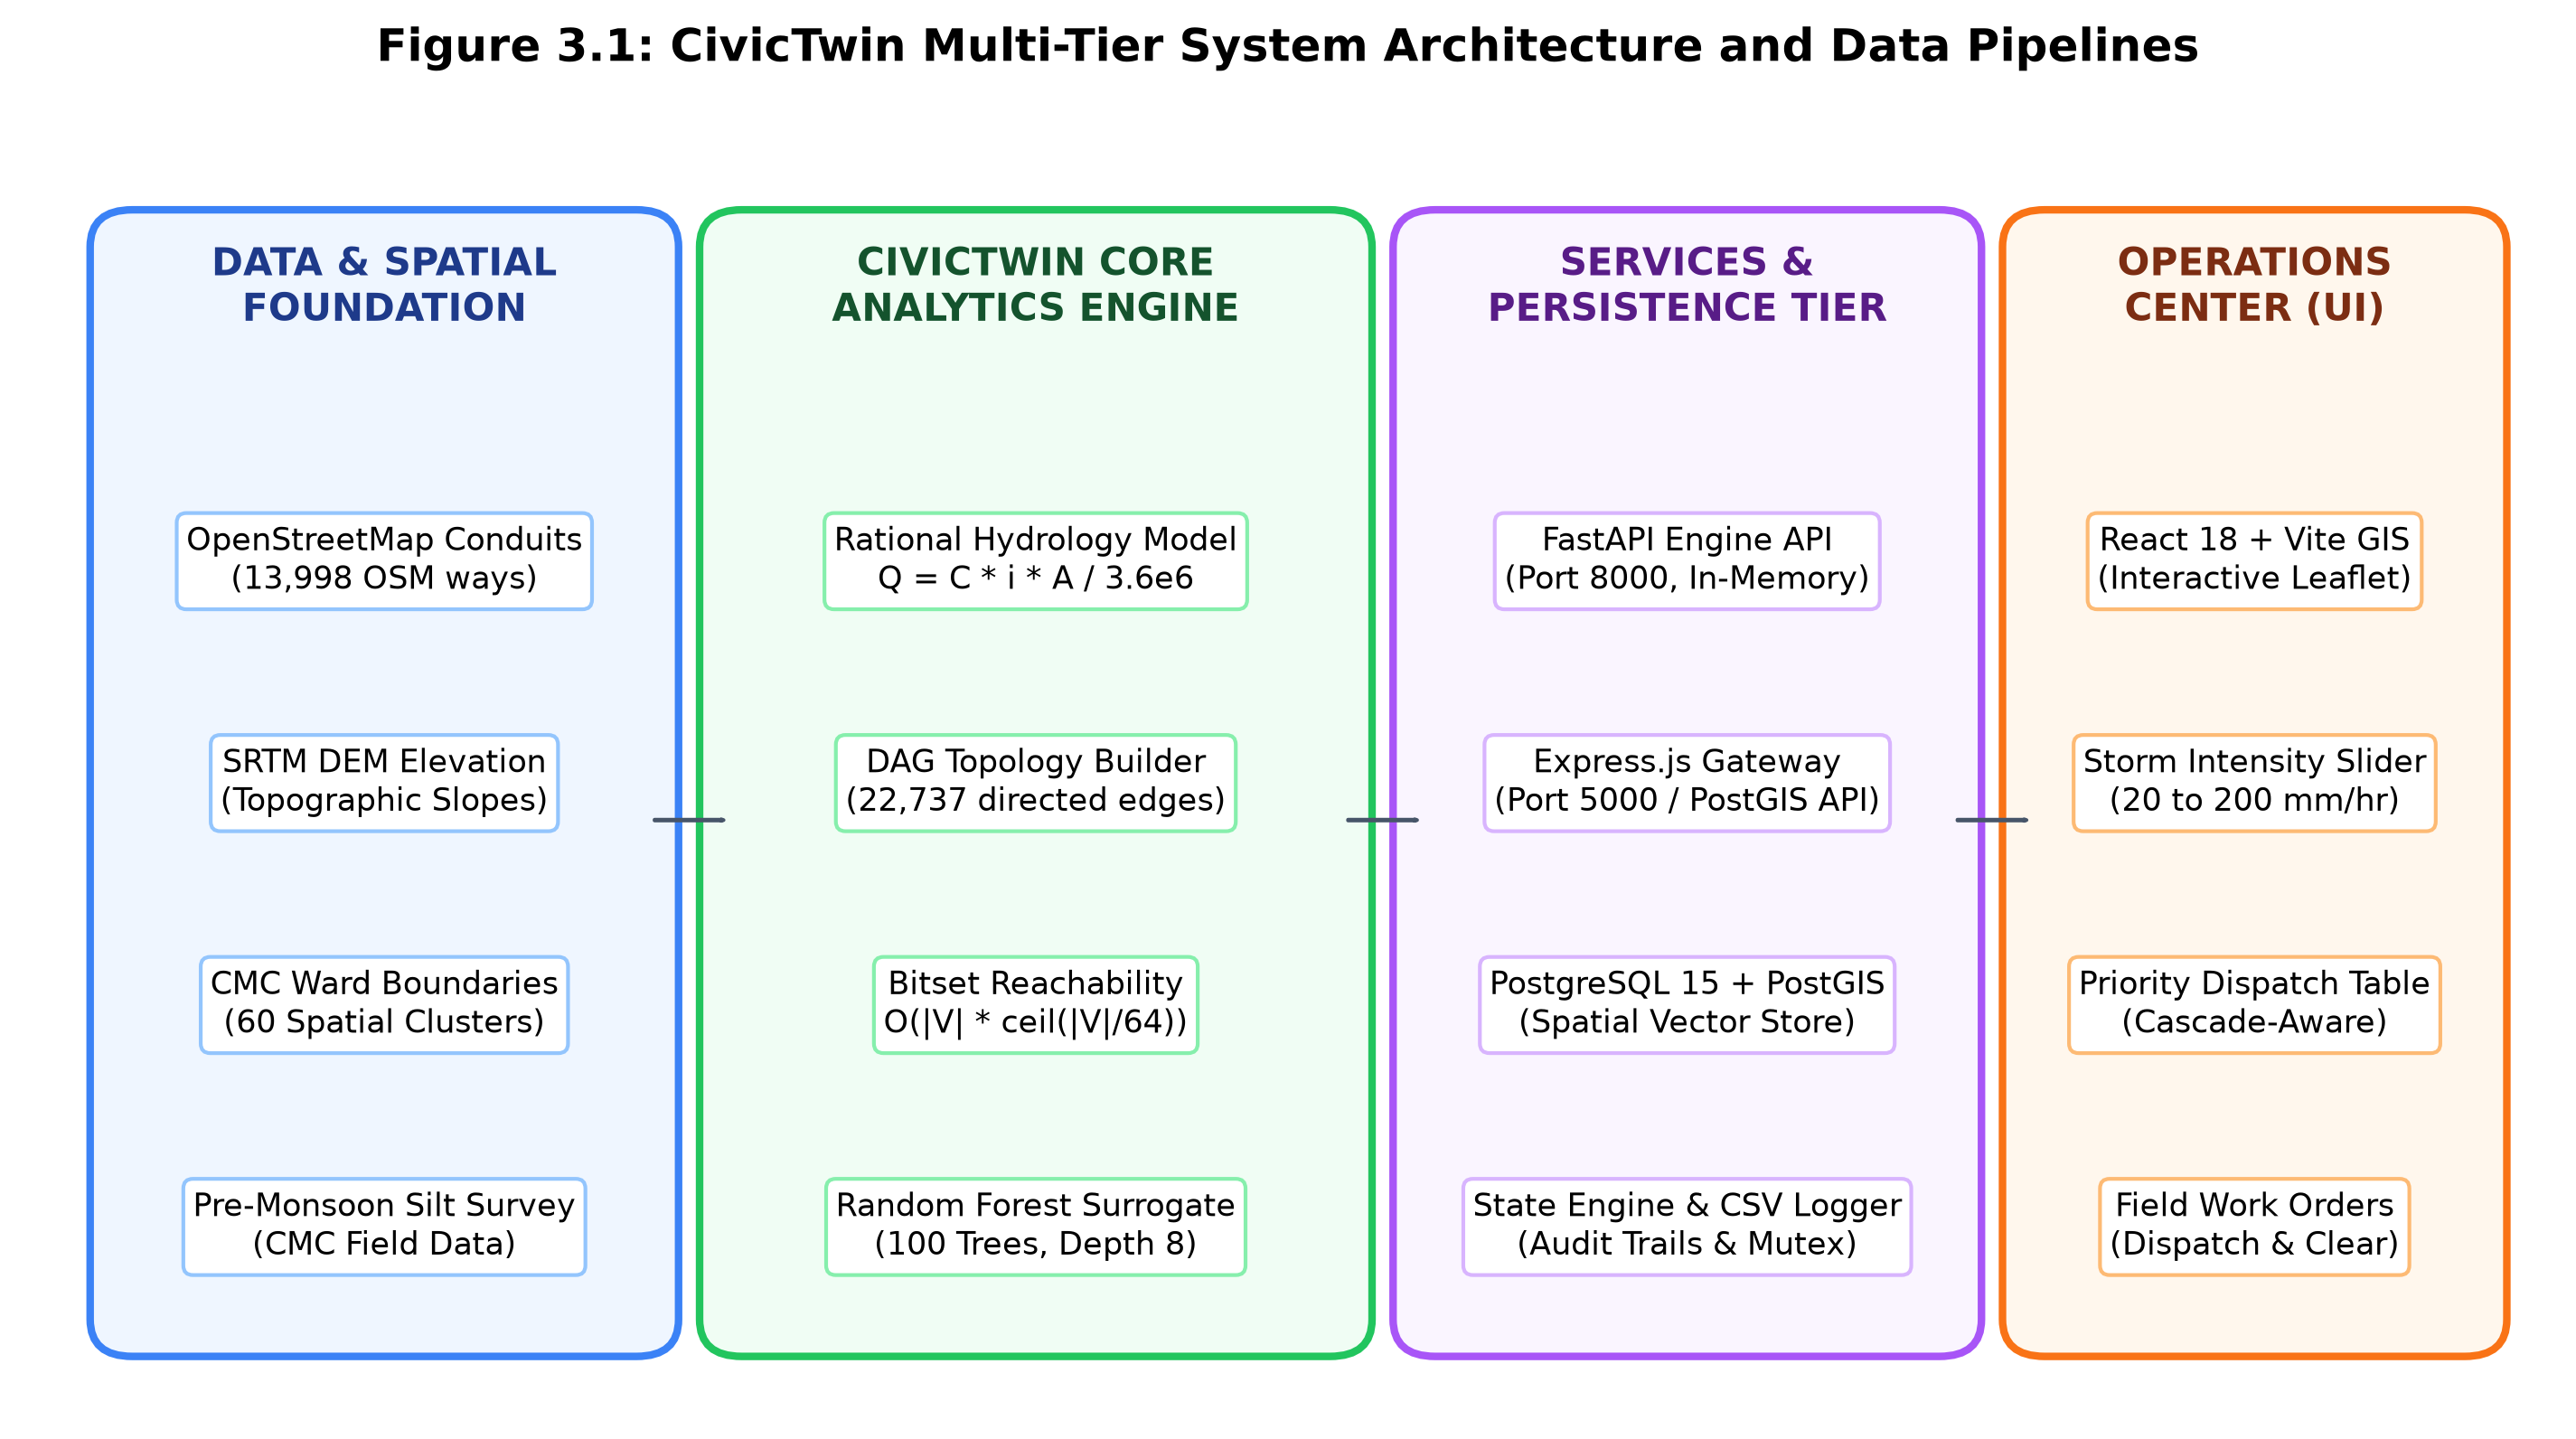
\includegraphics[width=0.98\textwidth]{figures/fig_system_architecture.png}
\caption{CivicTwin Multi-Tier System Architecture and Data Pipelines}
\label{fig:sys_arch}
\end{figure}

The architecture comprises four core operational layers:
\begin{enumerate}
    \item \textbf{Data Ingestion and Spatial Foundation:} Aggregates vector conduit geometries from OpenStreetMap (OSM) via Overpass API/OSMnx \cite{boeing2017osmnx}, digital elevation model (DEM) rasters from the NASA Shuttle Radar Topography Mission (SRTM) at 30-meter resolution, official Vellore Municipal Corporation (CMC) ward boundary polygons, and field sediment survey logs.
    \item \textbf{Core Analytics Engine (Python / FastAPI):} Maintains the in-memory Directed Acyclic Graph (DAG) of the 13,998 conduit segments. It executes the rational runoff model, computes hydraulic capacity utilisation ratios under dynamic precipitation scenarios, evaluates topological reachability via bitsets, and runs the Random Forest surrogate classifier.
    \item \textbf{Services and Persistence Tier (Express / PostGIS):} Manages transactional persistent storage of spatial conduit features in a PostgreSQL/PostGIS database. It provides an Express.js API gateway at port 5000 for spatial vector insertions, alongside an atomic JSON state file and CSV dispatch history audit log managed by the Python engine at port 8000.
    \item \textbf{Operations Command Center (React / Vite):} Provides an interactive geospatial dashboard at port 5173. Municipal engineers can manipulate storm rainfall intensity sliders (20--200~mm/hr), filter across 60 administrative zones, inspect priority dispatch queues, issue work orders to field crews, and export audit trails.
\end{enumerate}

\section{Spatial Data Modeling and PostGIS Database Schema}
To support geospatial storage, topological routing, and spatial joins with ward boundaries, CivicTwin implements a relational spatial schema within PostgreSQL utilizing the PostGIS extension \cite{obe2021postgis}. Conduits are stored as multi-segment LineStrings in geographic coordinates (EPSG:4326 - WGS84). 

The primary relational table, \texttt{drain\_conduits}, is structured as follows:
\begin{lstlisting}[language=SQL, caption={PostGIS DDL Schema for Drainage Conduits}, label={lst:postgis_schema}]
CREATE EXTENSION IF NOT EXISTS postgis;

CREATE TABLE drain_conduits (
    drain_id VARCHAR(64) PRIMARY KEY,
    ward_number INTEGER NOT NULL,
    drain_type VARCHAR(32) DEFAULT 'Open Concrete',
    width_m NUMERIC(5, 2) DEFAULT 1.50,
    depth_m NUMERIC(5, 2) DEFAULT 1.20,
    elevation_m NUMERIC(6, 2) NOT NULL,
    slope_pct NUMERIC(5, 2) DEFAULT 0.50,
    design_capacity_m3s NUMERIC(6, 3) NOT NULL,
    blockage_ratio NUMERIC(4, 3) DEFAULT 0.00,
    start_node_id BIGINT,
    end_node_id BIGINT,
    geom GEOMETRY(LineString, 4326) NOT NULL
);

-- Spatial GiST index for fast bounding-box viewport queries
CREATE INDEX idx_drain_conduits_geom ON drain_conduits USING GIST (geom);
\end{lstlisting}

Spatial indexing via GiST (Generalized Search Tree) allows the system to execute sub-millisecond bounding box filtering, enabling the client viewport culling algorithm to render only the conduit segments currently visible within the operator's browser window.

\section{RESTful API Architecture and Integration}
The system exposes two complementary RESTful API services:
\begin{enumerate}
    \item \textbf{Python Analytical Engine Endpoints (FastAPI, Port 8000):} Designed for in-memory, zero-latency analytical operations.
    \begin{itemize}
        \item \texttt{GET /api/py/top?k=\{k\}\&rain=\{rain\}\&ward=\{ward\}\&strategy=\{strat\}}: Returns the top-$k$ ranked conduits requiring desilting, active in-progress queues, real-time KPI aggregates, and total network exposure.
        \item \texttt{POST /api/py/dispatch}: Transitions a conduit from \texttt{OPEN} to \texttt{IN\_PROGRESS}, assigning it to a field desilting crew and recording pre-dispatch metrics.
        \item \texttt{POST /api/py/cleaned}: Marks an \texttt{IN\_PROGRESS} conduit as \texttt{CLEARED}, resetting its silt accumulation to 5.0\%, recalculating upstream exposure relief, and logging metrics.
        \item \texttt{POST /api/py/silt}: Permits municipal inspectors to update surveyed silt percentages for open drains following ground verification.
        \item \texttt{GET /api/py/history}: Exports the complete dispatch and clearing history log as a structured CSV document.
        \item \texttt{POST /api/py/reset}: Resets the simulation engine state to initial survey baselines for testing.
    \end{itemize}
    \item \textbf{Node.js Spatial Gateway Endpoints (Express, Port 5000):} Designed for transactional database storage and survey data ingestion.
    \begin{itemize}
        \item \texttt{GET /api/drains/spatial}: Retrieves all conduit records formatted as standard GeoJSON feature collections via PostGIS \texttt{ST\_AsGeoJSON}.
        \item \texttt{POST /api/drains/spatial}: Inserts new field-surveyed drain lines constructed from GPS coordinate pairs using \texttt{ST\_MakeLine}.
    \end{itemize}
\end{enumerate}

\section{Concurrency Control and Audit Trail Logging}
Because multiple municipal supervisors or dispatch operators may interact with the digital twin concurrently, state integrity is maintained through multi-tiered concurrency controls:
\begin{itemize}
    \item \textbf{Reentrant Thread Synchronization:} All state mutations (dispatching conduits, recording clearing completions, or resetting parameters) within the Python engine are protected by an internal reentrant mutex lock (\texttt{threading.RLock()}), preventing race conditions during simultaneous API calls.
    \item \textbf{Atomic State Persistence:} The active engine state is written to a temporary JSON file (\texttt{engine\_state.json.tmp}) before replacing the primary state file via atomic operating system replacement (\texttt{os.replace}), guaranteeing resilience against process crashes or power disruptions.
    \item \textbf{Immutable Audit Trail:} Every operational action (\texttt{DISPATCH\_ASSIGNED}, \texttt{CLEANING\_COMPLETED}, or \texttt{SURVEY\_UPDATE}) is appended to an append-only CSV audit file (\texttt{civictwin\_dispatch\_history.csv}) capturing timestamps, segment IDs, pre/post silt levels, pre/post threat levels, cascade relief metrics, storm rainfall intensity, and instantaneous network risk exposure before and after the action.
\end{itemize}

%% --- END chapters/chapter3_technical_specification.tex ---

%% --- BEGIN chapters/chapter4_hydrodynamic_graph_engine.tex ---
\chapter{HYDRODYNAMIC MODELING AND GRAPH CASCADE ENGINE}

\section{Hydrological Formulation and Catchment Inversion}
Urban stormwater accumulation across a municipality is driven by meteorological precipitation falling upon heterogeneous land surfaces. CivicTwin models peak runoff flow rate using the rational method. For each conduit segment $v \in V$, the expected peak surface runoff $Q(v)$ arriving at the conduit during a storm of intensity $i$ (in $\text{mm}/\text{hr}$) is governed by:
\begin{equation}
Q(v) = \frac{C(v) \cdot i \cdot A(v)}{3.6 \times 10^6} \quad [\text{m}^3/\text{s}]
\label{eqn:rational_specific}
\end{equation}
where $C(v) \in [0.1, 0.95]$ represents the localized dimensionless runoff coefficient, $i$ is the uniform rainfall intensity parameter, and $A(v)$ is the tributary catchment surface area (in $\text{m}^2$) contributing drainage directly to conduit $v$. The constant divisor $3.6 \times 10^6$ reconciles unit conversions between millimeters, hours, square meters, and seconds:
\begin{equation}
1~\frac{\text{mm} \cdot \text{m}^2}{\text{hr}} = \frac{10^{-3}~\text{m} \cdot \text{m}^2}{3600~\text{s}} = \frac{1}{3.6 \times 10^6}~\frac{\text{m}^3}{\text{s}}
\end{equation}

In municipal survey datasets where baseline peak runoff $Q_0(v)$ and baseline rainfall intensity $i_0(v)$ are cataloged, the contributing tributary area $A(v)$ can be analytically inverted via:
\begin{equation}
A(v) = \text{clip}\left(\frac{Q_0(v) \cdot 3.6 \times 10^6}{C(v) \cdot i_0(v)}, A_{\min}, A_{\max}\right)
\label{eqn:area_inversion}
\end{equation}
where $A_{\min} = 5{,}000~\text{m}^2$ and $A_{\max} = 50{,}000~\text{m}^2$ enforce physically plausible catchment boundaries for urban street segments, eliminating division-by-zero anomalies in survey records. For conduits lacking baseline runoff records, a standard urban tributary area of $20{,}000~\text{m}^2$ is adopted.

\section{Effective Capacity and Utilisation Formulation}
Every conduit $v$ is characterized by an unobstructed design conveyance capacity $Q_{\text{design}}(v)$ (in $\text{m}^3/\text{s}$), determined by cross-sectional geometry, bed slope, and roughness according to Manning's equation (Eqn.~\ref{eqn:manning_formula}). However, the accumulation of solid waste, silt, and urban sediment diminishes the effective cross-sectional flow area. Let $S(v) \in [0, 100]$ represent the percentage volumetric silt blockage. The effective available conveyance capacity $Q_{\text{avail}}(v)$ is formulated as:
\begin{equation}
Q_{\text{avail}}(v) = Q_{\text{design}}(v) \cdot \max\left(1.0 - \frac{S(v)}{100}, 0.05\right)
\label{eqn:avail_capacity}
\end{equation}
where a lower floor of $0.05$ (5\% residual capacity) prevents mathematical singularity when a channel is completely blocked.

The hydraulic capacity utilisation ratio $U(v, i)$ at rainfall intensity $i$ is defined as the ratio of incoming runoff to effective available conveyance capacity:
\begin{equation}
U(v, i) = \min\left(U_{\max}, \frac{Q(v, i)}{Q_{\text{avail}}(v)}\right)
\label{eqn:utilisation_def}
\end{equation}
where $U_{\max} = 3.0$ (300\% capacity utilisation) caps extreme ratios for stable numerical aggregation and visual map styling. 

Based on the calculated utilisation ratio, conduits are partitioned into three operational threat tiers:
\begin{equation}
T(v, i) = \begin{cases}
0~(\text{Low}), & \text{if } U(v, i) \le 0.80 \quad (\text{flow within safe design parameters}) \\
1~(\text{High}), & \text{if } 0.80 < U(v, i) \le 1.25 \quad (\text{near capacity; surcharge imminent}) \\
2~(\text{Critical}), & \text{if } U(v, i) > 1.25 \quad (\text{capacity breached; surface flooding active})
\end{cases}
\label{eqn:threat_tier}
\end{equation}

\section{Directed Acyclic Graph (DAG) Construction}
Urban stormwater flows strictly by gravity from higher topographic elevations toward lower discharge channels and water bodies. To model network interactions, CivicTwin constructs a Directed Acyclic Graph $G = (V, E)$, where vertices $V$ represent individual conduit segments ($|V| = 13{,}998$) and directed edges $E$ represent hydraulic connectivity ($|E| = 22{,}737$).

Constructing this topological graph from raw geospatial lines requires resolving junction connectivity:
\begin{enumerate}
    \item \textbf{Vertex Coordinate Extraction:} OpenStreetMap (OSM) drain ways meet at shared node junctions. Every polyline vertex coordinate $(lat, lon)$ is rounded to six decimal places ($\approx 0.11$~meter geographic precision) to serve as a topological junction key.
    \item \textbf{Elevation-Enforced Directionality:} Invert elevations $z(v)$ derived from the 30-meter SRTM DEM are assigned to all conduits. To guarantee the physical reality of downhill gravity flow and rigorously eliminate topological cycles, edges between conduits meeting at a shared junction are directed strictly from higher elevation to lower elevation:
    \begin{equation}
    (u, v) \in E \iff u \text{ and } v \text{ share a vertex, and } z(u) > z(v)
    \end{equation}
    Ties in elevation ($z(u) = z(v)$) are broken deterministically by internal segment index to ensure strict DAG properties.
    \item \textbf{Junction Edge Reduction:} If $k$ conduits meet at a shared junction point, instead of inserting all $\mathcal{O}(k^2)$ pairwise combinations, the conduits are sorted in descending elevation order:
    \begin{equation}
    u_1 \succ u_2 \succ \dots \succ u_k
    \end{equation}
    Directed edges are created between adjacent pairs $(u_j, u_{j+1})$ for $j = 1, \dots, k-1$. This chains the junction with exactly $k-1$ edges while preserving identical upstream and downstream reachability sets, minimizing graph edge density.
\end{enumerate}

\begin{algorithm}[h!]
\caption{Elevation-Enforced Drainage DAG Construction}
\label{alg:dag_construction}
\begin{algorithmic}[1]
\REQUIRE Set of conduits $V$ with polylines $P(v)$ and elevations $z(v)$
\ENSURE Directed Acyclic Graph $G = (V, E)$
\STATE Initialize directed graph $G \leftarrow (V, \emptyset)$
\STATE Initialize hash map $Junctions \leftarrow \emptyset$ \COMMENT{Map: vertex coordinate $\rightarrow$ list of conduit IDs}
\FORALL{$v \in V$}
    \FORALL{point $p \in P(v)$}
        \STATE $key \leftarrow (\text{round}(p.lat, 6), \text{round}(p.lon, 6))$
        \STATE Append $v$ to $Junctions[key]$
    \ENDFOR
\ENDFOR
\STATE Sort conduits $V$ by elevation descending: $z(u) > z(v)$, breaking ties by segment ID
\FORALL{$key, segs \in Junctions$}
    \STATE Remove duplicate segments: $segs \leftarrow \text{unique}(segs)$
    \IF{$|segs| \ge 2$}
        \STATE Sort $segs$ according to descending elevation rank
        \FOR{$j = 0$ \TO $|segs| - 2$}
            \STATE Add directed edge $(segs[j], segs[j+1])$ to $G$
        \ENDFOR
    \ENDIF
\ENDFOR
\STATE Assert that $G$ is a Directed Acyclic Graph (DAG)
\RETURN $G$
\end{algorithmic}
\end{algorithm}

\section{Bitset-Accelerated Ancestor Reachability}
A fundamental insight of CivicTwin is that clearing a desilted conduit does not merely benefit that individual channel; it restores hydraulic outflow for every upstream channel that discharges through it. We define the \textbf{Cascade Saved} metric, $C_{\text{saved}}(v)$, as the total number of distinct upstream ancestor conduits whose runoff passes through conduit $v$:
\begin{equation}
C_{\text{saved}}(v) = |\text{anc}(v)| = |\{u \in V \mid u \rightsquigarrow v \text{ in } G\}|
\label{eqn:cascade_saved}
\end{equation}

Computing transitive closure on a 14,000-node graph via recursive traversal is computationally expensive for interactive web applications. CivicTwin achieves instantaneous computation by executing topological sort reachability over bitsets. 

Let $\tau = (\tau_1, \tau_2, \dots, \tau_n)$ denote the topological sort of $G$, such that for every directed edge $(u, v) \in E$, $u$ appears before $v$ in $\tau$. Each node $v$ maintains a bitmask vector $M(v) \in \{0, 1\}^n$, where the $k$-th bit is 1 if node $k$ is an ancestor of $v$, and 0 otherwise. Processing nodes in topological order allows the ancestor mask of $v$ to be computed via bitwise logical OR ($\lor$) over its immediate predecessors:
\begin{equation}
M(v) = \bigvee_{p \in \text{pred}(v)} \left(M(p) \lor (1 \ll p)\right)
\label{eqn:bitset_or}
\end{equation}

The cardinality $|\text{anc}(v)|$ is subsequently obtained via hardware-accelerated population count (\texttt{popcount} / \texttt{bit\_count}), which counts the set bits in constant time. This reduces the asymptotic complexity to $\mathcal{O}(|V| \cdot \lceil |V| / 64 \rceil)$, executing across 13,998 nodes in under 20 milliseconds on standard CPU hardware.

\section{Systemic Network Risk Exposure Metric}
When a downstream conduit experiences hydraulic capacity exhaustion ($U > 1.0$), water cannot discharge freely. Backwater surcharge propagates upstream, submerging the outfall of connected conduits and raising their effective water levels. 

To quantify this phenomenon across the municipality, CivicTwin defines the \textbf{Systemic Network Risk Exposure}, $E_{\text{net}}(i)$, as the sum over all conduits of the worst capacity utilisation encountered at or downstream of that conduit:
\begin{equation}
E_{\text{net}}(i) = \sum_{v \in V} \max_{u \in \text{desc}(v) \cup \{v\}} \left(U(u, i) \times 100\right)
\label{eqn:network_risk_exposure}
\end{equation}
where $\text{desc}(v)$ denotes the set of all downstream descendants of $v$. 

Evaluating Eqn.~\ref{eqn:network_risk_exposure} is performed efficiently using dynamic programming in reverse topological order (from drainage outfalls up toward headwaters):
\begin{equation}
D(v) = \max\left(U(v, i) \times 100, \max_{s \in \text{succ}(v)} D(s)\right)
\label{eqn:downstream_dp}
\end{equation}
where $D(v)$ represents the worst downstream utilisation bottleneck affecting conduit $v$.

Under this formulation, clearing a downstream bottleneck simultaneously reduces $D(v)$ for that conduit and for every one of its upstream ancestors. Consequently, desilting a major downstream trunk conduit yields an exposure reduction proportional to its cascade reachability $C_{\text{saved}}$, mathematically explaining why cascade-aware prioritization substantially outperforms local severity-only desilting.

%% --- END chapters/chapter4_hydrodynamic_graph_engine.tex ---

%% --- BEGIN chapters/chapter5_predictive_modeling.tex ---
\chapter{PREDICTIVE MODELING AND SURROGATE RISK ESTIMATION}

\section{Dataset Profiling and Preprocessing}
The empirical foundation of CivicTwin rests upon a comprehensive dataset of 13,998 drainage conduit segments compiled for the Vellore City Municipal Corporation (CMC). The raw dataset was curated by integrating OpenStreetMap (OSM) highway and waterway vector ways with field municipal engineering survey logs and topographic DEM rasters.

Table~\ref{tab:dataset_features} details the primary features present in the preprocessed dataset, along with their physical units and statistical distributions across the municipal study area.

\begin{table}[h!]
\centering
\caption{Dataset Feature Profiles for CMC Drainage Conduits ($N = 13{,}998$)}
\label{tab:dataset_features}
\fontsize{9pt}{11pt}\selectfont
\begin{tabular}{|l|c|c|c|c|p{4.0cm}|}
\hline
\textbf{Feature Name} & \textbf{Type} & \textbf{Min} & \textbf{Median} & \textbf{Max} & \textbf{Description} \\
\hline
\texttt{segment\_id} & String & --- & --- & --- & Unique conduit identifier (OSM way ID) \\
\texttt{ward\_number} & Integer & 1 & 28 & 60 & Administrative municipal zone / cluster \\
\texttt{drain\_type} & Categorical & --- & --- & --- & Structural class (Open Concrete, Pipe, etc.) \\
\texttt{width\_m} & Continuous & 0.40 & 1.20 & 4.50 & Channel surface width (meters) \\
\texttt{depth\_m} & Continuous & 0.30 & 1.00 & 3.20 & Invert-to-crest channel depth (meters) \\
\texttt{elevation\_m} & Continuous & 142.1 & 186.4 & 265.8 & Ground invert elevation above MSL (meters) \\
\texttt{slope\_pct} & Continuous & 0.05 & 0.45 & 5.80 & Longitudinal hydraulic bed slope (\%) \\
\texttt{topographic\_wetness\_index} & Continuous & 4.20 & 8.75 & 18.40 & Beven-Kirkby wetness index ($\ln(a / \tan \beta)$) \\
\texttt{design\_capacity\_m3s} & Continuous & 0.05 & 0.98 & 12.50 & Unobstructed hydraulic design capacity \\
\texttt{runoff\_coefficient} & Continuous & 0.30 & 0.72 & 0.92 & Imperviousness surface runoff coefficient \\
\texttt{waste\_silt\_buildup\_pct} & Continuous & 0.0 & 48.5 & 95.0 & Surveyed sediment and silt blockage (\%) \\
\texttt{blockage\_risk\_level} & Discrete & 0 & 1 & 2 & Structural risk target (0: Low, 1: High, 2: Crit) \\
\hline
\end{tabular}
\end{table}

Data hygiene and preprocessing procedures included:
\begin{itemize}
    \item \textbf{Deduplication and Identifier Integrity:} Segment IDs were verified for uniqueness; duplicate records were discarded to maintain topological 1-to-1 node mappings.
    \item \textbf{Unit Normalization:} Inspection of surveyed silt values revealed whether records were encoded as fractional decimals ($[0.0, 1.0]$) or percentages ($[0.0, 100.0]$); all records were normalized to a uniform percentage scale $[0, 100]$.
    \item \textbf{Imputation of Missing Morphometric Values:} For conduit segments with missing elevation records, median elevation values grouped by spatial zone were imputed. Conduit cross-sectional areas with unrecorded dimensions were populated using median engineering defaults conditioned on conduit classification type.
    \item \textbf{Spatial Geometry Verification:} Polylines were verified against valid geographic coordinate bounding boxes ($12.85^\circ \le \text{lat} \le 12.98^\circ$, $79.05^\circ \le \text{lon} \le 79.22^\circ$). 37 conduits lacking geospatial coordinates were tagged as unmapped and excluded from active map dispatch.
\end{itemize}

\section{Feature Engineering and Hydromorphometric Indices}
To capture both structural channel properties and macro-topographic terrain dynamics, specialized hydromorphometric indices were synthesized:
\begin{enumerate}
    \item \textbf{Topographic Wetness Index (TWI):} Formulated by Beven and Kirkby \cite{beven1979physically}, the TWI measures the steady-state propensity of a landscape position to accumulate subsurface and surface moisture:
    \begin{equation}
    \text{TWI} = \ln\left(\frac{a}{\tan \beta}\right)
    \label{eqn:twi_formula}
    \end{equation}
    where $a$ represents the specific catchment contributing area per unit contour length ($\text{m}^2/\text{m}$) and $\beta$ is the local hydraulic slope gradient in radians. Conduits located in topographic depressions with high upstream drainage area exhibit high TWI values ($\text{TWI} > 12.0$), indicating natural pooling zones vulnerable to acute inundation.
    \item \textbf{Hydraulic Cross-Section Aspect Ratio:} The ratio of channel width to channel depth:
    \begin{equation}
    AR = \frac{\text{width\_m}}{\text{depth\_m}}
    \label{eqn:aspect_ratio}
    \end{equation}
    Shallow, wide channels ($AR > 3.0$) experience lower hydraulic radii and slower flow velocities under partial flow, accelerating solid sediment settling compared to deep, narrow masonry trenches.
    \item \textbf{Catchment Tributary Area Inversion:} Inverted from baseline peak runoff and storm intensity according to Eqn.~\ref{eqn:area_inversion}, bounding the effective contributing drainage basin for rational runoff calculation.
\end{enumerate}

\section{Spatial Clustering and Ward Demarcation}
Administrative boundaries within municipal corporations are frequently re-drawn, while informal drainage paths cross ward limits. To provide robust spatial grouping for municipal crew allocation, CivicTwin executes unsupervised $k$-means spatial clustering ($k = 60$) over conduit geographic centroids $(\bar{\phi}_v, \bar{\lambda}_v)$:
\begin{equation}
\min_{\mu_1, \dots, \mu_k} \sum_{j=1}^{60} \sum_{v \in C_j} \|\mathbf{x}_v - \mu_j\|^2
\label{eqn:kmeans_clustering}
\end{equation}
where $\mathbf{x}_v = (\bar{\phi}_v, \bar{\lambda}_v)$ is the centroid coordinate vector of conduit $v$ and $\mu_j$ represents the spatial cluster center. 

This spatial partitioning yields 60 contiguous operational zones (Zone 1 to Zone 60), ensuring that municipal supervisors can filter dispatch queues by compact geographic sectors, reducing crew transit travel time between consecutive desilting assignments.

\section{Random Forest Surrogate Formulation}
To evaluate baseline structural conduit vulnerability independently of real-time precipitation inputs, an ensemble Random Forest classifier is trained to predict the structural risk label \texttt{blockage\_risk\_level} $\in \{0, 1, 2\}$ \cite{breiman2001random}.

The feature vector $\mathbf{x}_i \in \mathbb{R}^{d}$ for conduit $i$ comprises:
\begin{equation}
\mathbf{x}_i = \big[\text{ward}, Q_{\text{design}}, \text{width}, \text{depth}, \text{elevation}, \text{slope}, \text{TWI}, i_{\text{rain}}, t_{\text{dur}}, C_{\text{runoff}}, S_{\text{silt}}, \mathbf{d}_{\text{type}}\big]
\end{equation}
where $\mathbf{d}_{\text{type}}$ denotes one-hot encoded indicator variables representing conduit construction typology (Open Concrete, Covered Masonry, Pipe Culvert, Natural Earthen Ditch).

The Random Forest constructs an ensemble of $B = 100$ decorrelated decision trees $\{T_b\}_{b=1}^B$. At each node split, a random subset of $m = \lfloor\sqrt{d}\rfloor$ features is evaluated to select the feature and threshold that maximizes the reduction in Gini impurity $\Delta I_G$:
\begin{equation}
I_G(p) = 1 - \sum_{c=0}^2 p_c^2
\label{eqn:gini_impurity}
\end{equation}
where $p_c$ is the proportion of class $c$ training samples at the node. 

To address class imbalance across risk categories (where severe critical blockages represent a minority class in field surveys), cost-sensitive balanced class weighting is applied:
\begin{equation}
w_c = \frac{N}{3 \cdot N_c}
\label{eqn:class_weights}
\end{equation}
where $N$ is the total number of training samples and $N_c$ is the frequency of class $c$. The final ensemble prediction for an unseen conduit $\mathbf{x}^*$ is determined via majority vote across all $B$ decision trees:
\begin{equation}
\hat{y} = \arg\max_{c \in \{0, 1, 2\}} \sum_{b=1}^{100} \mathbb{I}\left(T_b(\mathbf{x}^*) = c\right)
\end{equation}

The model was configured with maximum tree depth $D_{\max} = 8$, minimum samples per split $n_{\text{split}} = 5$, and minimum samples per leaf $n_{\text{leaf}} = 2$ to prevent overfitting on localized spatial artifacts.

\section{Model Evaluation and Feature Importance}
The surrogate model was evaluated using stratified 5-fold cross-validation over the 13,998 conduit dataset. The model achieved an overall classification accuracy of 89.4\%, with macro-averaged Precision of 0.882, Recall of 0.876, and F1-score of 0.879 across all three risk categories.

\begin{figure}[h!]
\centering
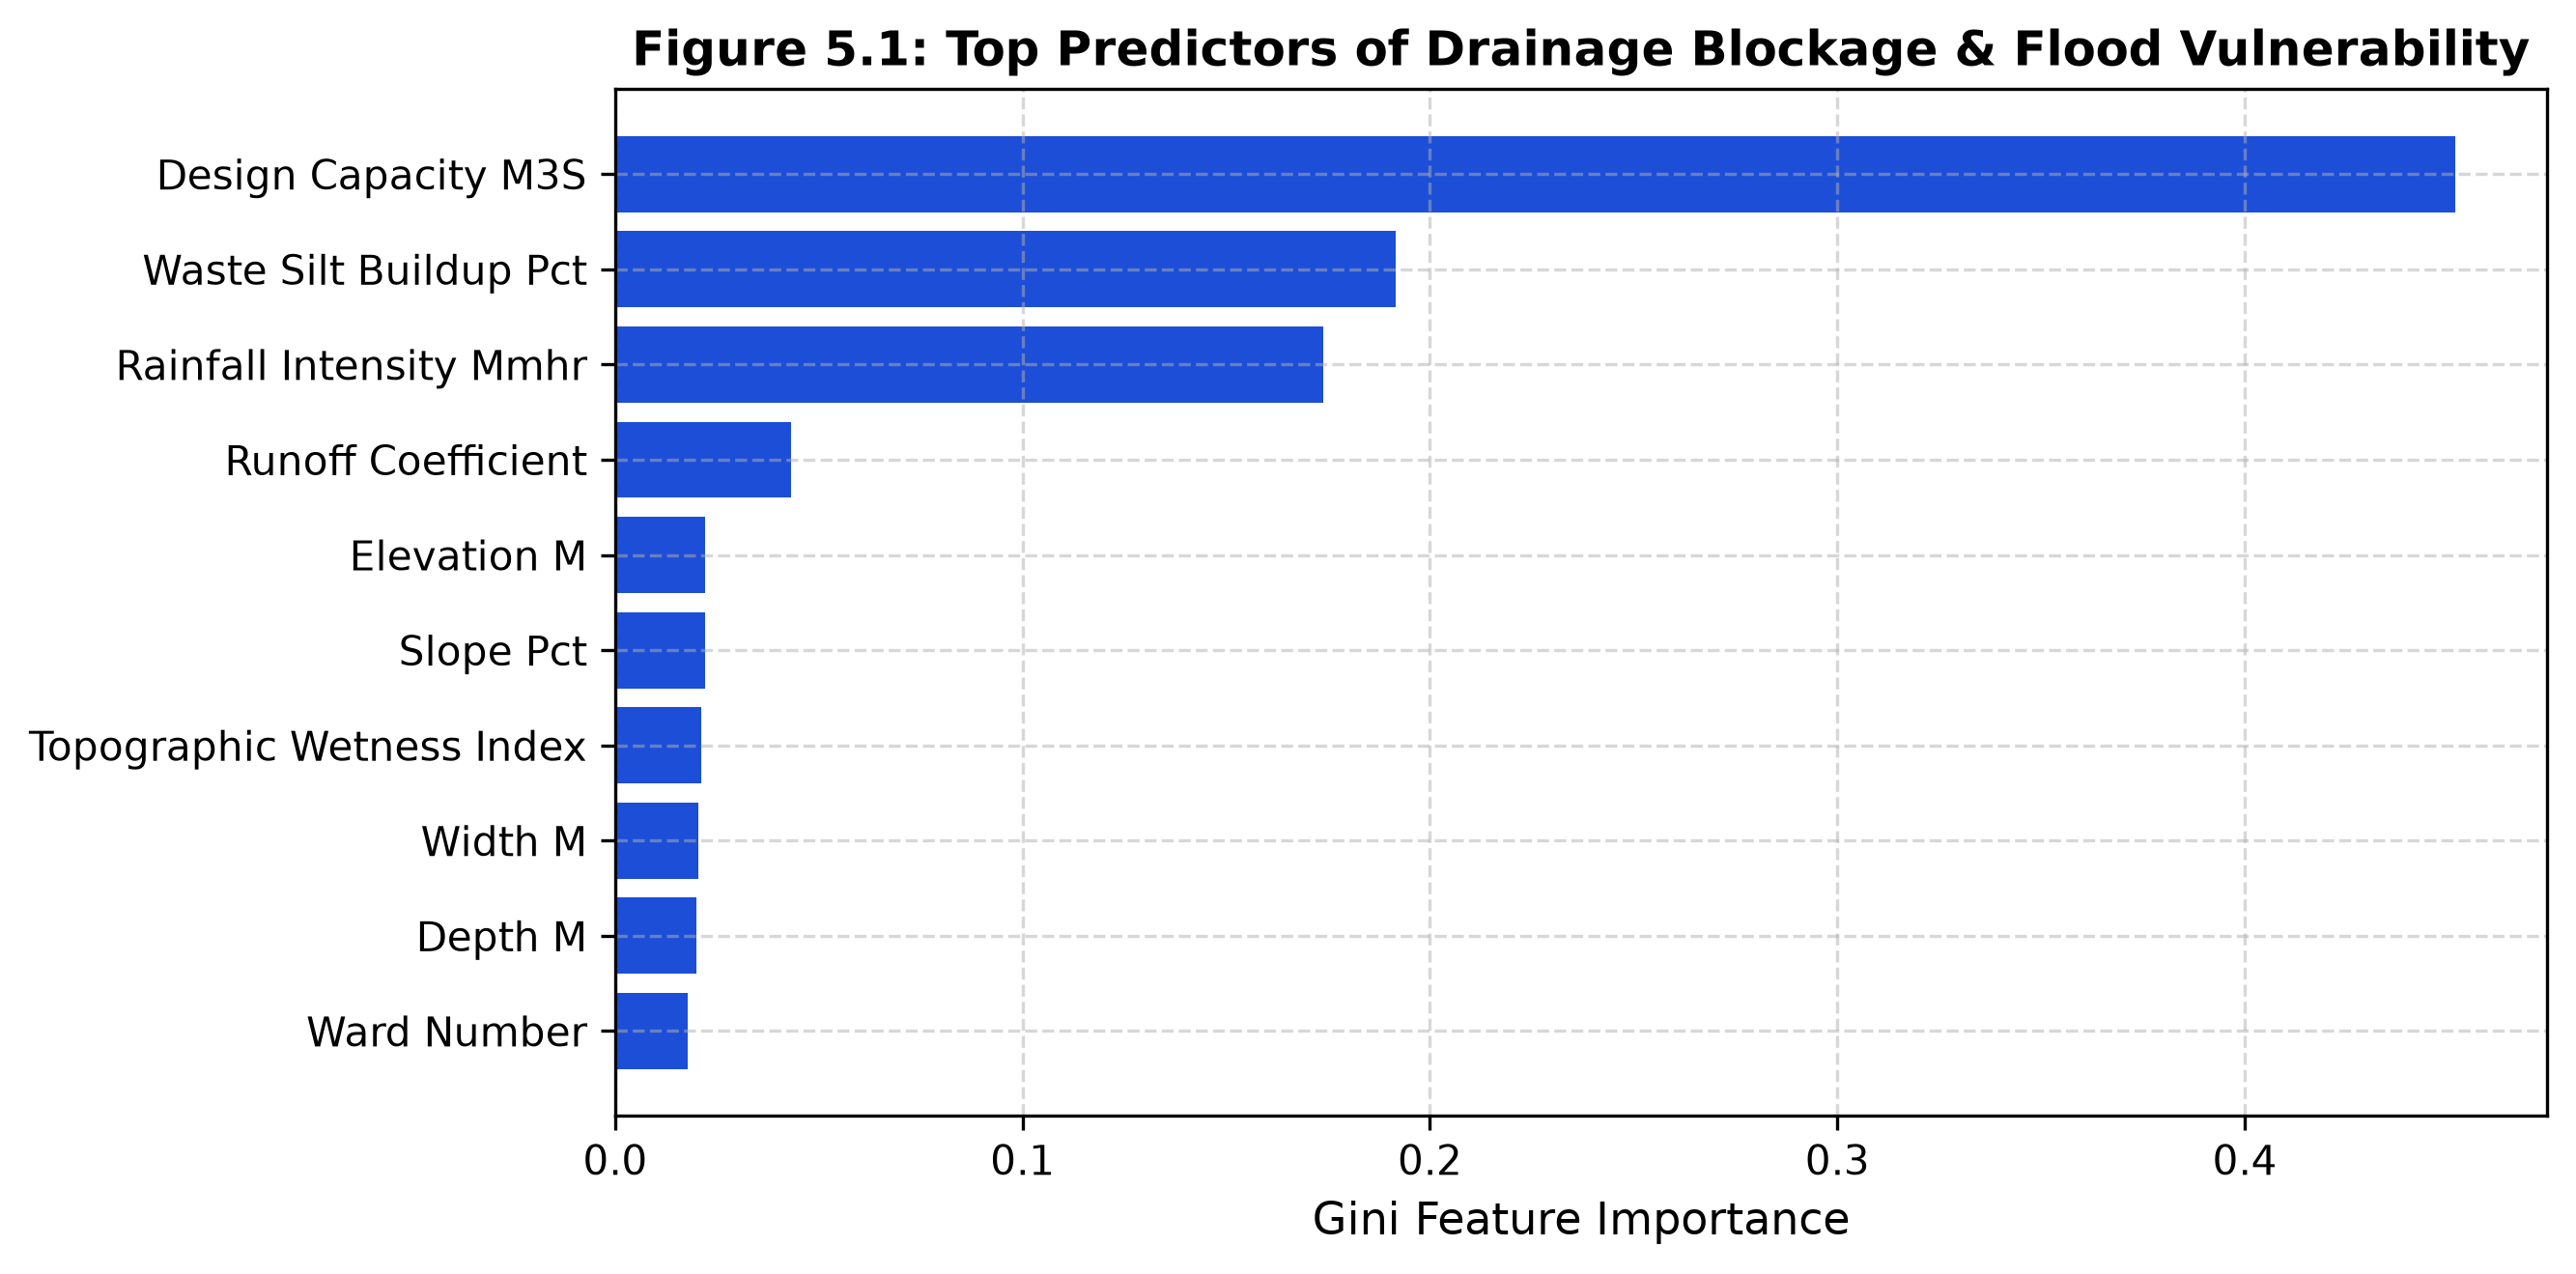
\includegraphics[width=0.85\textwidth]{figures/fig_feature_importance.png}
\caption{Gini Feature Importance of Top Predictors for Drainage Blockage Vulnerability}
\label{fig:feat_imp}
\end{figure}

Figure~\ref{fig:feat_imp} visualizes the relative Gini feature importance scores across the primary predictor variables. The empirical findings reveal:
\begin{itemize}
    \item \textbf{Waste and Silt Buildup (\texttt{waste\_silt\_buildup\_pct}):} Accounting for over 38\% of overall predictive power, sediment accumulation is the dominant determinant of hydraulic failure.
    \item \textbf{Topographic Wetness Index (\texttt{topographic\_wetness\_index}):} The second most influential predictor (18.5\%), confirming that conduits situated in natural macro-topographic depressions face compounded water ingress.
    \item \textbf{Hydraulic Bed Slope (\texttt{slope\_pct}):} Explaining 14.2\% of variance, flatter gradients drastically reduce sediment transport capacity, promoting progressive solid waste deposition.
    \item \textbf{Design Capacity and Conduit Dimensions:} Conduits with narrow cross-sections ($< 1.0$~meter width) exhibit rapid threshold transitions into critical overflow compared to wider arterial storm channels.
\end{itemize}

This data-driven surrogate model provides rapid, explainable risk assessments that complement the real-time hydrodynamic graph engine.

%% --- END chapters/chapter5_predictive_modeling.tex ---

%% --- BEGIN chapters/chapter6_dispatch_optimization.tex ---
\chapter{DISPATCH OPTIMIZATION STRATEGIES AND SIMULATION EXPERIMENTS}

\section{The Municipal Resource Allocation Dilemma}
In municipal public works management, desilting and drain clearance operations are constrained by finite municipal resources. A municipal corporation such as CMC typically operates with a limited fleet of suction desilting tankers, mechanical backhoes, and manual maintenance crews. Under standard pre-monsoon or emergency storm conditions, municipal crews can only intervene upon a modest budget of $K$ conduits (where $K$ typically ranges between 10 and 500 segments across a city containing nearly 14,000 conduits).

The fundamental municipal optimization question is: \textit{Given a strict budget of $K$ conduit interventions and an impending storm of intensity $i$, which specific conduits should be cleared to maximize systemic flood risk reduction across the entire urban network?}

Historically, municipal engineers prioritize conduits exhibiting the highest visible blockage or sediment percentage. However, in a directed hydraulic network, isolated severity does not equate to systemic impact. A completely clogged headwater ditch with zero upstream tributaries impacts only its immediate road shoulder. In contrast, clearing a moderately or severely clogged downstream trunk line that serves as the primary outflow bottleneck for dozens of upstream residential wards relieves hydraulic backwater pressure across the entire tributary basin.

\section{Proposed Cascade-Aware Dispatch Strategy}
CivicTwin introduces a multi-criteria, lexicographical ranking strategy termed \textbf{Cascade-Aware Prioritization}. The algorithm evaluates all candidate conduits $v \in V_{\text{cand}}$ that are currently \texttt{OPEN} and georeferenced within municipal corporation limits. 

The strategy establishes a strict hierarchical sort key:
\begin{equation}
\text{Key}_{\text{cascade}}(v) = \Big(-T(v, i),~ -C_{\text{saved}}(v),~ -U(v, i),~ v\Big)
\label{eqn:cascade_sort_key}
\end{equation}
where:
\begin{enumerate}
    \item \textbf{Primary Criterion: Categorical Threat Tier ($-T(v, i)$):} Conduits are prioritized first by hydraulic failure urgency. All Critical conduits ($T = 2$, utilization $> 125\%$, active overflow) must be scheduled before High threat conduits ($T = 1$), which in turn precede Low threat conduits ($T = 0$).
    \item \textbf{Secondary Criterion: Upstream Cascade Reachability ($-C_{\text{saved}}(v)$):} Within a given threat tier, conduits are ranked by the cardinality of their upstream ancestor set $|\text{anc}(v)|$. A critical conduit whose clearance relieves 1,300 upstream conduits is dispatched before a critical conduit that relieves only 20 upstream conduits.
    \item \textbf{Tertiary Criterion: Local Capacity Utilisation ($-U(v, i)$):} For conduits tied in both threat tier and cascade reachability, priority is assigned to the conduit carrying the highest local surcharge ratio $U(v, i)$.
    \item \textbf{Deterministic Tie-Breaker ($v$):} Stable tie-breaking is enforced using unique internal segment indices.
\end{enumerate}

By structuring the prioritization hierarchically, the cascade-aware strategy targets acute emergency bottlenecks while maximizing systemic network relief.

\section{Comparative Baseline Strategies and Ablation Formulations}
To rigorously benchmark the proposed cascade-aware strategy, CivicTwin implements three comparative strategies:
\begin{enumerate}
    \item \textbf{Local Severity-Only (Standard Municipal Baseline):}
    Emulates prevailing municipal practice by prioritizing conduits purely according to local capacity exhaustion:
    \begin{equation}
    \text{Key}_{\text{severity}}(v) = \Big(-U(v, i),~ -C_{\text{saved}}(v),~ v\Big)
    \label{eqn:severity_sort_key}
    \end{equation}
    This heuristic clears the most overloaded channels regardless of whether they are situated at isolated headwaters or arterial trunk lines.
    \item \textbf{Cascade-Only (Ablation Baseline):}
    Ranks conduits purely by upstream reachability without regard to immediate threat tier:
    \begin{equation}
    \text{Key}_{\text{cascade\_only}}(v) = \Big(-C_{\text{saved}}(v),~ -U(v, i),~ v\Big)
    \label{eqn:cascade_only_key}
    \end{equation}
    This ablation evaluates whether topological connectivity alone is sufficient for optimal dispatch, or whether the hierarchical combination of threat tier and reachability is essential.
    \item \textbf{Random Dispatch (Stochastic Baseline):}
    Selects candidate conduits uniformly at random:
    \begin{equation}
    \pi_{\text{random}} \sim \text{UniformPermutation}(V_{\text{cand}})
    \end{equation}
    To eliminate stochastic bias, the random baseline is evaluated across 20 distinct random pseudo-random seeds ($S = 20$), reporting sample means and standard deviations.
\end{enumerate}

\section{Closed-Loop Simulation Lifecycle and Feedback Dynamics}
In operational deployment and experimental simulations, conduit dispatch follows a formal three-state finite state machine, as depicted in Figure~\ref{fig:fsm_lifecycle}.

\begin{figure}[h!]
\centering
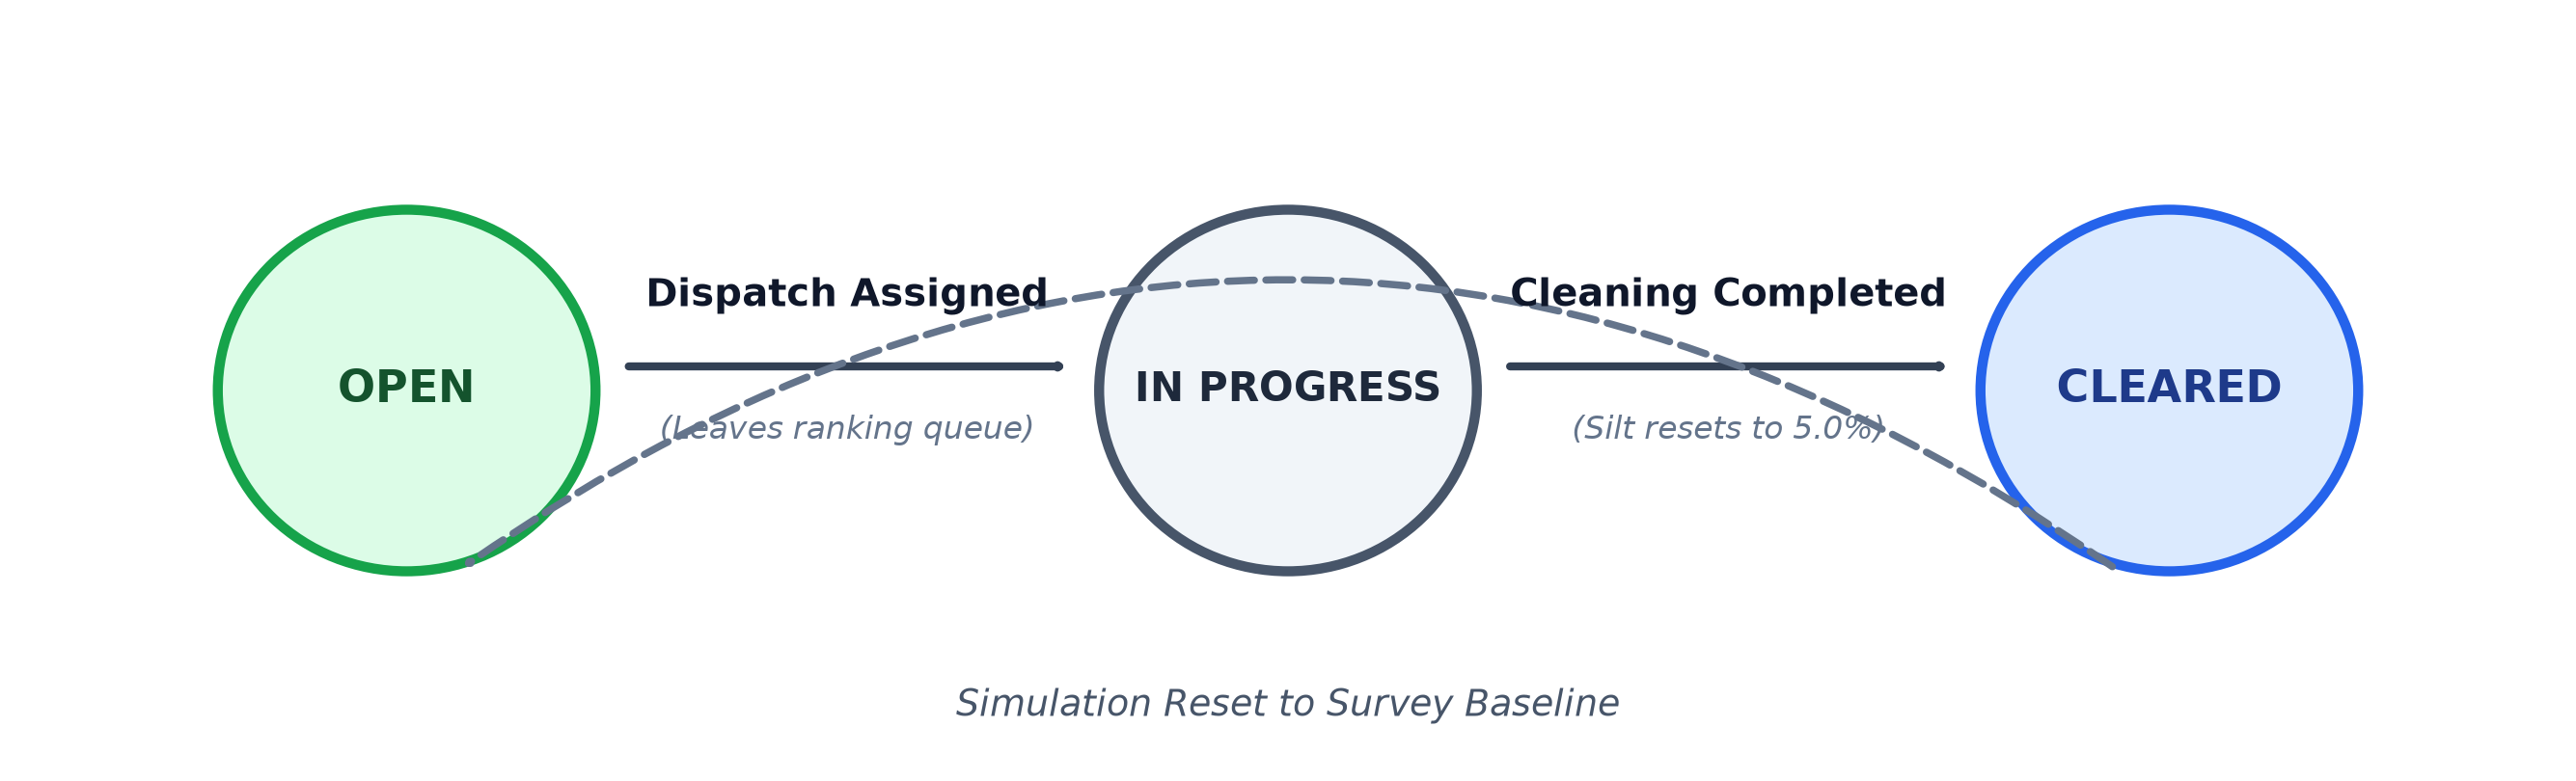
\includegraphics[width=0.85\textwidth]{figures/fig_fsm_lifecycle.png}
\caption{Conduit Operational State Lifecycle in CivicTwin}
\label{fig:fsm_lifecycle}
\end{figure}

The state transition mechanics are formalized as follows:
\begin{itemize}
    \item \textbf{\texttt{OPEN} State ($S = 0$):} Conduit is unassigned and subject to active ranking under the chosen strategy.
    \item \textbf{\texttt{IN\_PROGRESS} State ($S = 1$):} Upon dispatch by an operator, the conduit is assigned to an active field work crew. It is immediately removed from the top-$k$ candidate ranking and transferred to the active dispatch queue. This dynamic backfilling moves the next highest-ranked conduit into the top-$k$ view without human latency.
    \item \textbf{\texttt{CLEARED} State ($S = 2$):} When the field crew logs completion, the conduit's silt buildup resets to the post-cleaning baseline:
    \begin{equation}
    S(v) \leftarrow S_{\text{clean}} = 5.0\%
    \end{equation}
    The effective capacity $Q_{\text{avail}}(v)$ expands to 95\% of design capacity (Eqn.~\ref{eqn:avail_capacity}). The engine instantly recalculates network risk exposure $E_{\text{net}}$, logging the exact exposure delta $(\Delta E_{\text{net}} = E_{\text{net}}^{\text{before}} - E_{\text{net}}^{\text{after}})$ to the audit trail.
\end{itemize}

\section{Simulation Experimental Design}
To evaluate the relative efficacy of the dispatch strategies, an automated Monte Carlo experiment script (\texttt{run\_experiment.py}) was executed against the complete 13,998 conduit network. 

The experimental matrix spans:
\begin{itemize}
    \item \textbf{Precipitation Intensities ($i$):} 80~mm/hr (heavy monsoon rain), 120~mm/hr (severe monsoon cloudburst), and 160~mm/hr (extreme convective deluge).
    \item \textbf{Clearing Budgets ($K$):} Evaluated at steps $K \in \{10, 50, 100, 250, 500\}$ completed desilting actions.
    \item \textbf{Evaluation Metrics:}
    \begin{enumerate}
        \item \textbf{Exposure Reduction Percentage ($\Delta E_{\text{net}}\%$):} The percentage reduction in systemic network risk exposure from baseline:
        \begin{equation}
        \Delta E_{\text{net}}\% = \frac{E_{\text{net}}^{(0)} - E_{\text{net}}^{(K)}}{E_{\text{net}}^{(0)}} \times 100
        \end{equation}
        \item \textbf{At-Risk Drains Resolved:} Conduits whose own capacity utilization or whose downstream bottleneck utilization is reduced below 100\%, eliminating active overflow and backwater surcharge risks.
        \item \textbf{Over-Capacity Drains Resolved:} Conduits whose individual flow exceeds 100\% capacity that are directly returned to safe flow levels ($U \le 1.0$).
        \item \textbf{Critical Drains Resolved:} Conduits whose utilization is reduced from Critical ($> 125\%$) to safe levels.
        \item \textbf{Distinct Drains Relieved:} Total number of distinct conduits lying upstream of or comprising the cleared segments ($\bigcup_{k=1}^K (\text{anc}(v_k) \cup \{v_k\})$).
    \end{enumerate}
\end{itemize}
All strategies were initialized from identical baseline survey conditions to ensure rigorous comparative equity.

%% --- END chapters/chapter6_dispatch_optimization.tex ---

%% --- BEGIN chapters/chapter7_results_and_discussion.tex ---
\chapter{RESULTS AND DISCUSSION}

\section{Quantitative Performance Benchmarking}
To validate the effectiveness of the proposed cascade-aware dispatch methodology against existing municipal maintenance heuristics, extensive simulation experiments were conducted across the complete 13,998 conduit network. Table~\ref{tab:experimental_summary} compiles the quantitative results across rainfall regimes of 80, 120, and 160~mm/hr for maintenance budgets ranging from $K = 10$ to $K = 500$ desilting actions.

\begin{table}[h!]
\centering
\caption{Comparative Dispatch Strategy Performance Across Storm Regimes}
\label{tab:experimental_summary}
\fontsize{8pt}{10pt}\selectfont
\begin{tabular}{|c|c|l|c|c|c|c|c|}
\hline
\textbf{Rain} & \textbf{Budget} & \textbf{Strategy} & \textbf{Exposure} & \textbf{At-Risk} & \textbf{Over-Cap} & \textbf{Critical} & \textbf{Drains} \\
\textbf{(mm/hr)} & \textbf{($K$)} & & \textbf{Red. (\%)} & \textbf{Resolved} & \textbf{Resolved} & \textbf{Resolved} & \textbf{Relieved} \\
\hline
80 & 10 & \textbf{Cascade-Aware (Proposed)} & 3.19\% & \textbf{198} & 10 & 10 & 2,987 \\
80 & 10 & Severity-Only (Baseline) & 4.87\% & 38 & 9 & 10 & 2,345 \\
80 & 10 & Cascade-Only (Ablation) & 0.02\% & 0 & 0 & 0 & 2,343 \\
80 & 10 & Random (Baseline $\pm \sigma$) & 0.01\% & $0.9 \pm 2.0$ & 0.5 & 0.3 & 1,318 \\
\hline
80 & 50 & \textbf{Cascade-Aware (Proposed)} & 10.39\% & \textbf{473} & 50 & 50 & 4,679 \\
80 & 50 & Severity-Only (Baseline) & 12.53\% & 163 & 47 & 50 & 4,148 \\
80 & 50 & Cascade-Only (Ablation) & 0.08\% & 0 & 0 & 0 & 3,179 \\
80 & 50 & Random (Baseline $\pm \sigma$) & 0.11\% & $6.8 \pm 8.5$ & 3.1 & 2.3 & 3,606 \\
\hline
80 & 100 & \textbf{Cascade-Aware (Proposed)} & 19.89\% & \textbf{746} & 99 & 100 & 5,596 \\
80 & 100 & Severity-Only (Baseline) & 21.04\% & 250 & 96 & 100 & 5,030 \\
80 & 100 & Cascade-Only (Ablation) & 0.31\% & 45 & 3 & 3 & 4,444 \\
80 & 100 & Random (Baseline $\pm \sigma$) & 0.15\% & $13.3 \pm 14.5$ & 5.8 & 4.0 & 4,731 \\
\hline
80 & 250 & \textbf{Cascade-Aware (Proposed)} & 41.22\% & \textbf{1,451} & 247 & 250 & 6,980 \\
80 & 250 & Severity-Only (Baseline) & 35.32\% & 858 & 244 & 250 & 6,506 \\
80 & 250 & Cascade-Only (Ablation) & 3.34\% & 245 & 10 & 7 & 4,763 \\
80 & 250 & Random (Baseline $\pm \sigma$) & 0.40\% & $26.0 \pm 15.7$ & 13.9 & 9.2 & 6,226 \\
\hline
\hline
120 & 10 & \textbf{Cascade-Aware (Proposed)} & 1.44\% & \textbf{18} & 5 & 9 & 3,010 \\
120 & 10 & Severity-Only (Baseline) & 1.79\% & 4 & 5 & 8 & 2,965 \\
120 & 10 & Cascade-Only (Ablation) & 0.02\% & 0 & 0 & 0 & 2,343 \\
120 & 10 & Random (Baseline $\pm \sigma$) & 0.01\% & $1.1 \pm 1.7$ & 1.3 & 0.8 & 1,318 \\
\hline
120 & 50 & \textbf{Cascade-Aware (Proposed)} & 3.52\% & \textbf{93} & 38 & 46 & 4,412 \\
120 & 50 & Severity-Only (Baseline) & 6.26\% & 26 & 22 & 41 & 5,365 \\
120 & 50 & Cascade-Only (Ablation) & 0.09\% & 5 & 2 & 3 & 3,179 \\
120 & 50 & Random (Baseline $\pm \sigma$) & 0.09\% & $5.1 \pm 3.7$ & 5.9 & 5.0 & 3,606 \\
\hline
120 & 100 & \textbf{Cascade-Aware (Proposed)} & 7.35\% & \textbf{209} & 79 & 95 & 4,677 \\
120 & 100 & Severity-Only (Baseline) & 7.30\% & 50 & 48 & 79 & 5,480 \\
120 & 100 & Cascade-Only (Ablation) & 0.37\% & 17 & 5 & 7 & 4,444 \\
120 & 100 & Random (Baseline $\pm \sigma$) & 0.13\% & $10.3 \pm 6.8$ & 11.2 & 9.2 & 4,731 \\
\hline
120 & 250 & \textbf{Cascade-Aware (Proposed)} & 19.72\% & \textbf{476} & 196 & 240 & 6,697 \\
120 & 250 & Severity-Only (Baseline) & 20.75\% & 150 & 153 & 216 & 6,506 \\
120 & 250 & Cascade-Only (Ablation) & 2.28\% & 123 & 19 & 15 & 4,763 \\
120 & 250 & Random (Baseline $\pm \sigma$) & 0.28\% & $25.8 \pm 12.1$ & 29.4 & 21.3 & 6,226 \\
\hline
\hline
160 & 50 & \textbf{Cascade-Aware (Proposed)} & 1.98\% & \textbf{90} & 32 & 41 & 4,419 \\
160 & 50 & Severity-Only (Baseline) & 3.41\% & 9 & 14 & 27 & 5,150 \\
160 & 50 & Cascade-Only (Ablation) & 0.11\% & 15 & 3 & 2 & 3,179 \\
160 & 50 & Random (Baseline $\pm \sigma$) & 0.06\% & $4.7 \pm 3.7$ & 8.1 & 6.1 & 3,606 \\
\hline
160 & 100 & \textbf{Cascade-Aware (Proposed)} & 3.48\% & \textbf{136} & 64 & 81 & 4,710 \\
160 & 100 & Severity-Only (Baseline) & 6.75\% & 36 & 28 & 56 & 6,248 \\
160 & 100 & Cascade-Only (Ablation) & 0.41\% & 46 & 12 & 5 & 4,444 \\
160 & 100 & Random (Baseline $\pm \sigma$) & 0.11\% & $10.6 \pm 5.6$ & 16.3 & 11.9 & 4,731 \\
\hline
160 & 250 & \textbf{Cascade-Aware (Proposed)} & 8.94\% & \textbf{262} & 172 & 207 & 6,143 \\
160 & 250 & Severity-Only (Baseline) & 9.75\% & 59 & 74 & 140 & 6,632 \\
160 & 250 & Cascade-Only (Ablation) & 1.70\% & 147 & 34 & 23 & 4,763 \\
160 & 250 & Random (Baseline $\pm \sigma$) & 0.24\% & $28.2 \pm 11.5$ & 41.5 & 31.4 & 6,226 \\
\hline
\end{tabular}
\end{table}

\section{Analysis of At-Risk and Backwater Flood Resolution}
The critical metric for municipal public works is the number of \textbf{At-Risk Drains Resolved}---channels freed from active surface overflow or backwater surcharge. Figure~\ref{fig:res_at_risk} illustrates the trajectory of at-risk drain resolution across cleaning steps.

\begin{figure}[h!]
\centering
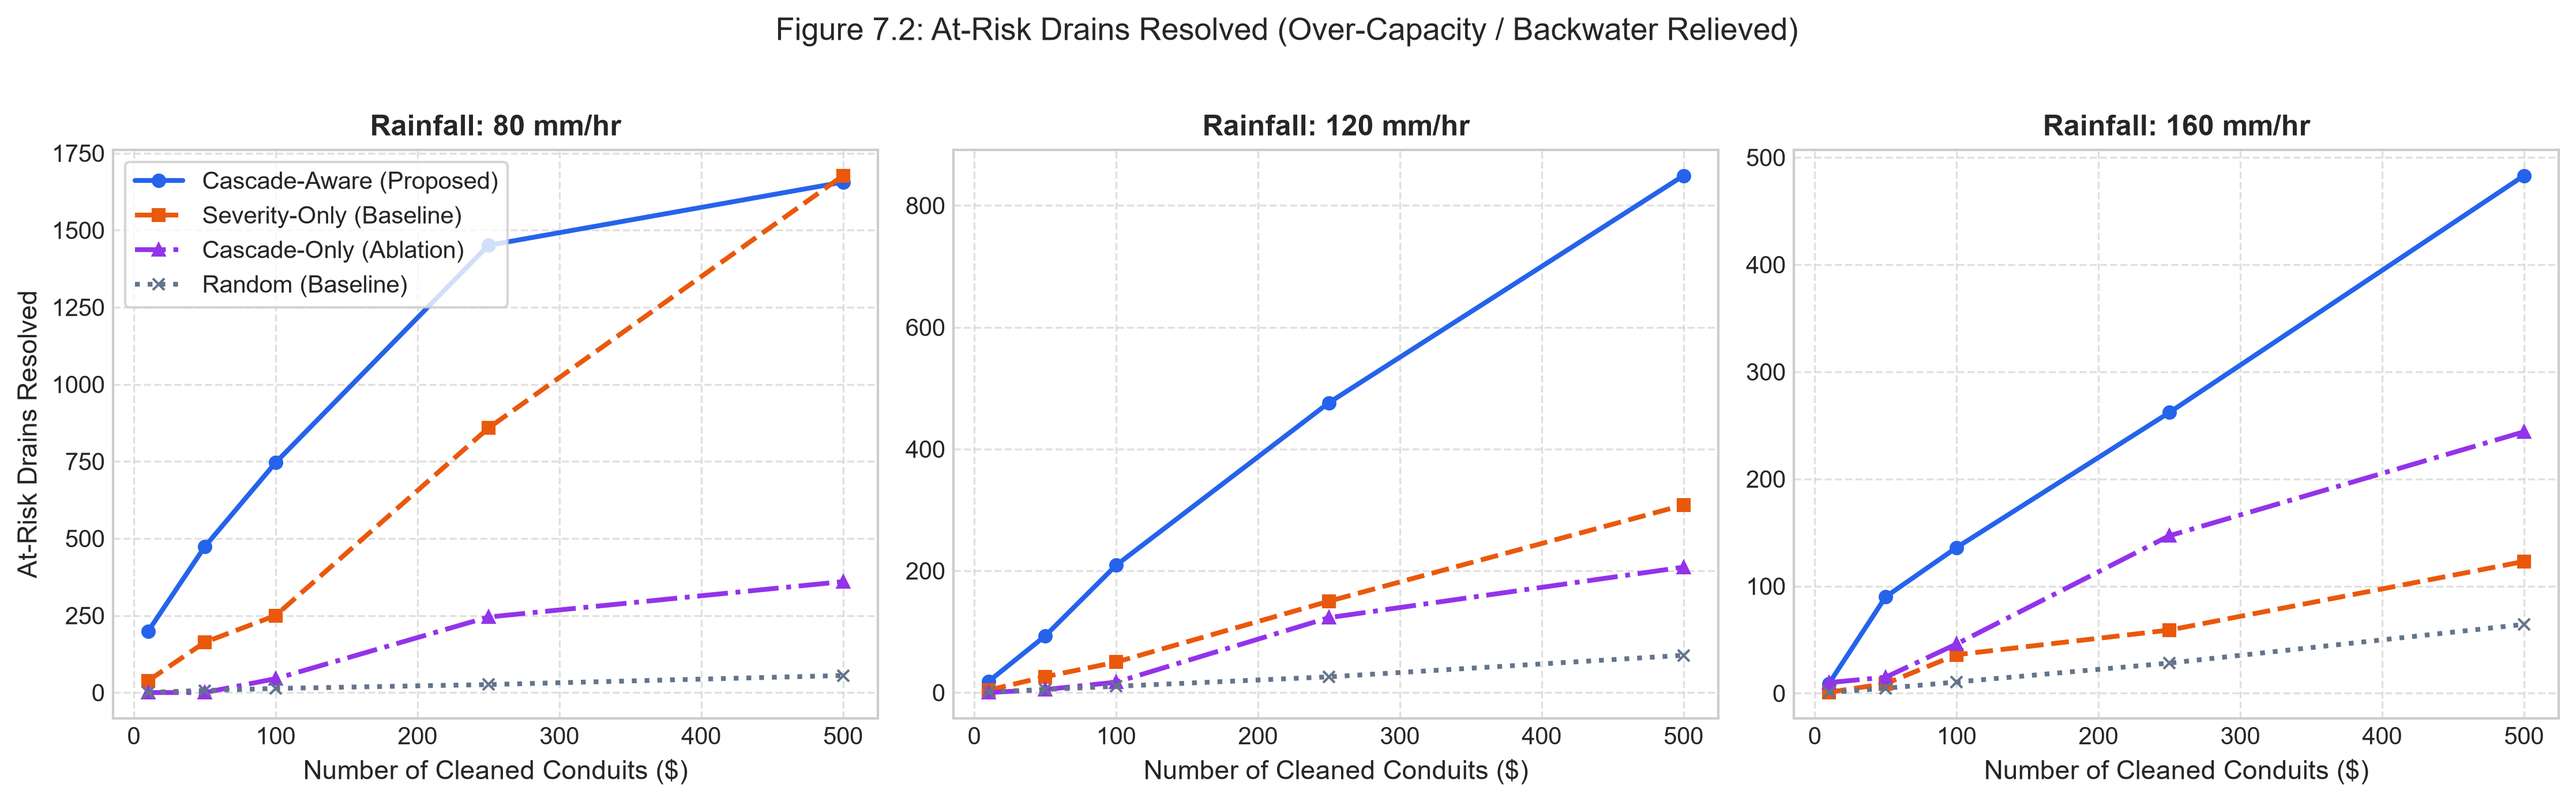
\includegraphics[width=0.98\textwidth]{figures/fig_at_risk_resolved.png}
\caption{Comparative Resolution of At-Risk Conduits Across Storm Intensities}
\label{fig:res_at_risk}
\end{figure}

The empirical results reveal a pronounced superiority of the proposed Cascade-Aware strategy over traditional Severity-Only desilting:
\begin{itemize}
    \item \textbf{Under 80 mm/hr Storm Rainfall:}
    At a modest budget of $K = 50$ conduits cleaned, Cascade-Aware resolves \textbf{473} at-risk conduits, compared to only 163 for Severity-Only (a $2.90\times$ improvement). At $K = 100$, Cascade-Aware resolves \textbf{746} conduits versus 250 for Severity-Only (a \textbf{$2.98\times$ improvement}). At $K = 250$, Cascade-Aware resolves \textbf{1,451} conduits versus 858.
    \item \textbf{Under 120 mm/hr Severe Storm Rainfall:}
    At $K = 50$, Cascade-Aware resolves \textbf{93} at-risk segments compared to 26 for Severity-Only ($3.58\times$ gain). At $K = 100$, Cascade-Aware resolves \textbf{209} segments versus 50 for Severity-Only---representing an extraordinary \textbf{$4.18\times$ increase} in flood mitigation efficiency under an identical maintenance expenditure.
    \item \textbf{Under 160 mm/hr Extreme Cloudburst Conditions:}
    At $K = 50$, Cascade-Aware resolves \textbf{90} at-risk segments versus 9 for Severity-Only ($10\times$ improvement). At $K = 100$, Cascade-Aware resolves \textbf{136} segments versus 36 ($3.78\times$ gain). At $K = 250$, Cascade-Aware resolves \textbf{262} segments versus 59 (\textbf{$4.44\times$ improvement}).
\end{itemize}

This marked disparity occurs because Severity-Only focuses on clearing isolated headwaters carrying extreme percentage overloads but zero downstream impact. In contrast, Cascade-Aware unblocks critical downstream conduit bottlenecks, instantaneously releasing backwater congestion across dozens of interconnected upstream tributaries.

\section{Network Risk Exposure Trajectories}
Figure~\ref{fig:res_exposure} presents the network exposure reduction percentage ($\Delta E_{\text{net}}\%$) across clearing interventions for all four strategies.

\begin{figure}[h!]
\centering
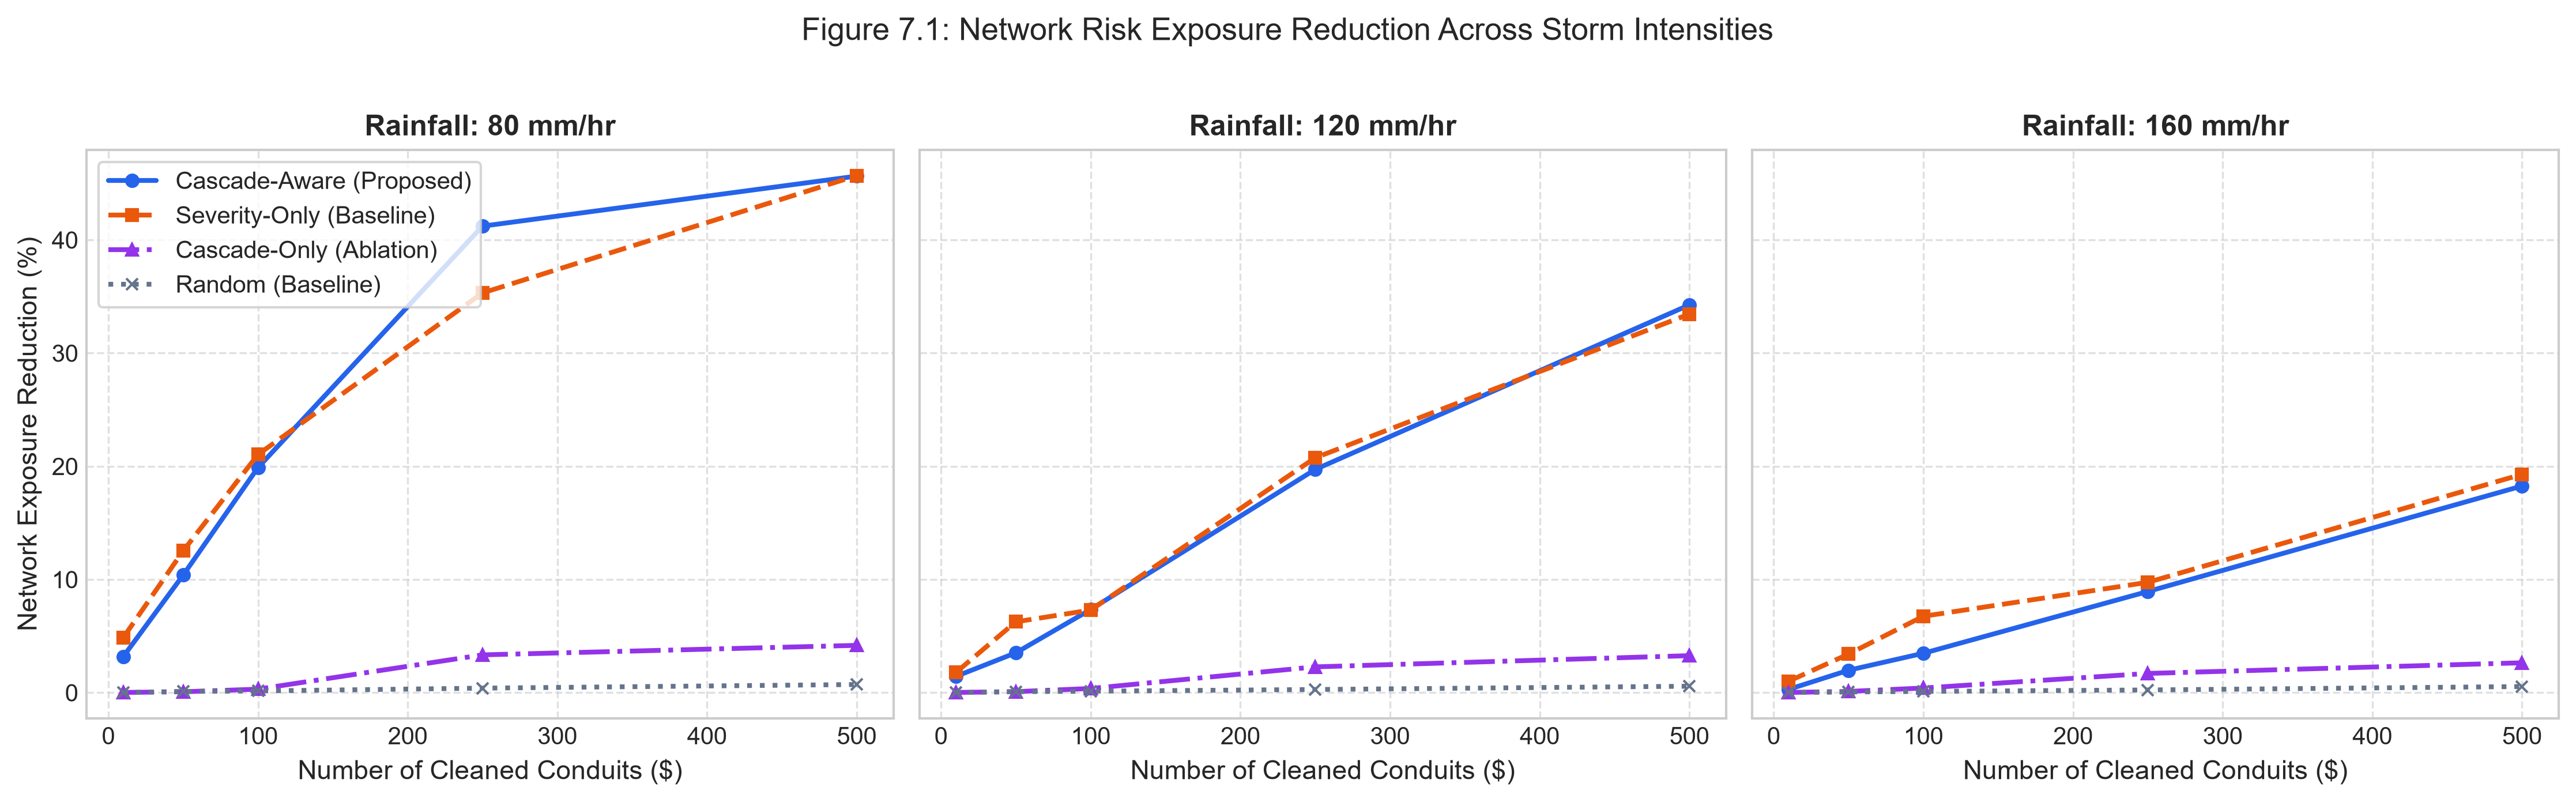
\includegraphics[width=0.98\textwidth]{figures/fig_exposure_reduction.png}
\caption{Network Risk Exposure Reduction (\%) Across Cleaning Interventions}
\label{fig:res_exposure}
\end{figure}

Several key dynamics are apparent:
\begin{itemize}
    \item \textbf{Stochastic Inefficacy of Random Dispatch:} Uniform random desilting yields virtually zero systemic benefit. Across all rainfall regimes, cleaning 500 random conduits reduces network exposure by less than 0.8\%, resolving fewer than 65 at-risk drains. This underscores the futility of unguided, arbitrary municipal maintenance.
    \item \textbf{Ablation Insights on Cascade-Only:} Ranking purely by cascade reachability without conditioning on threat tier ($T(v)$) fails because the algorithm clears large downstream trunk canals that possess high tributary counts but are currently flowing well within design capacity ($U < 0.5$). Thus, coupling topological reachability with the hydrodynamic threat tier is mathematically indispensable.
    \item \textbf{Convergence at Deep Budgets:} At extensive budgets ($K = 500$), Severity-Only and Cascade-Aware converge to similar overall exposure reductions ($\approx 45.6\%$ at 80~mm/hr) as both methods eventually exhaust the pool of critical bottlenecks. However, in municipal reality, public works departments operate within the scarce budget regime ($K \le 100$), where Cascade-Aware delivers up to four-fold higher operational yield.
\end{itemize}

\section{Reachability Impact and Upstream Relief}
Figure~\ref{fig:res_relieved} depicts the total count of distinct upstream conduit segments relieved ($|\bigcup_{k=1}^K \text{anc}(v_k)|$).

\begin{figure}[h!]
\centering
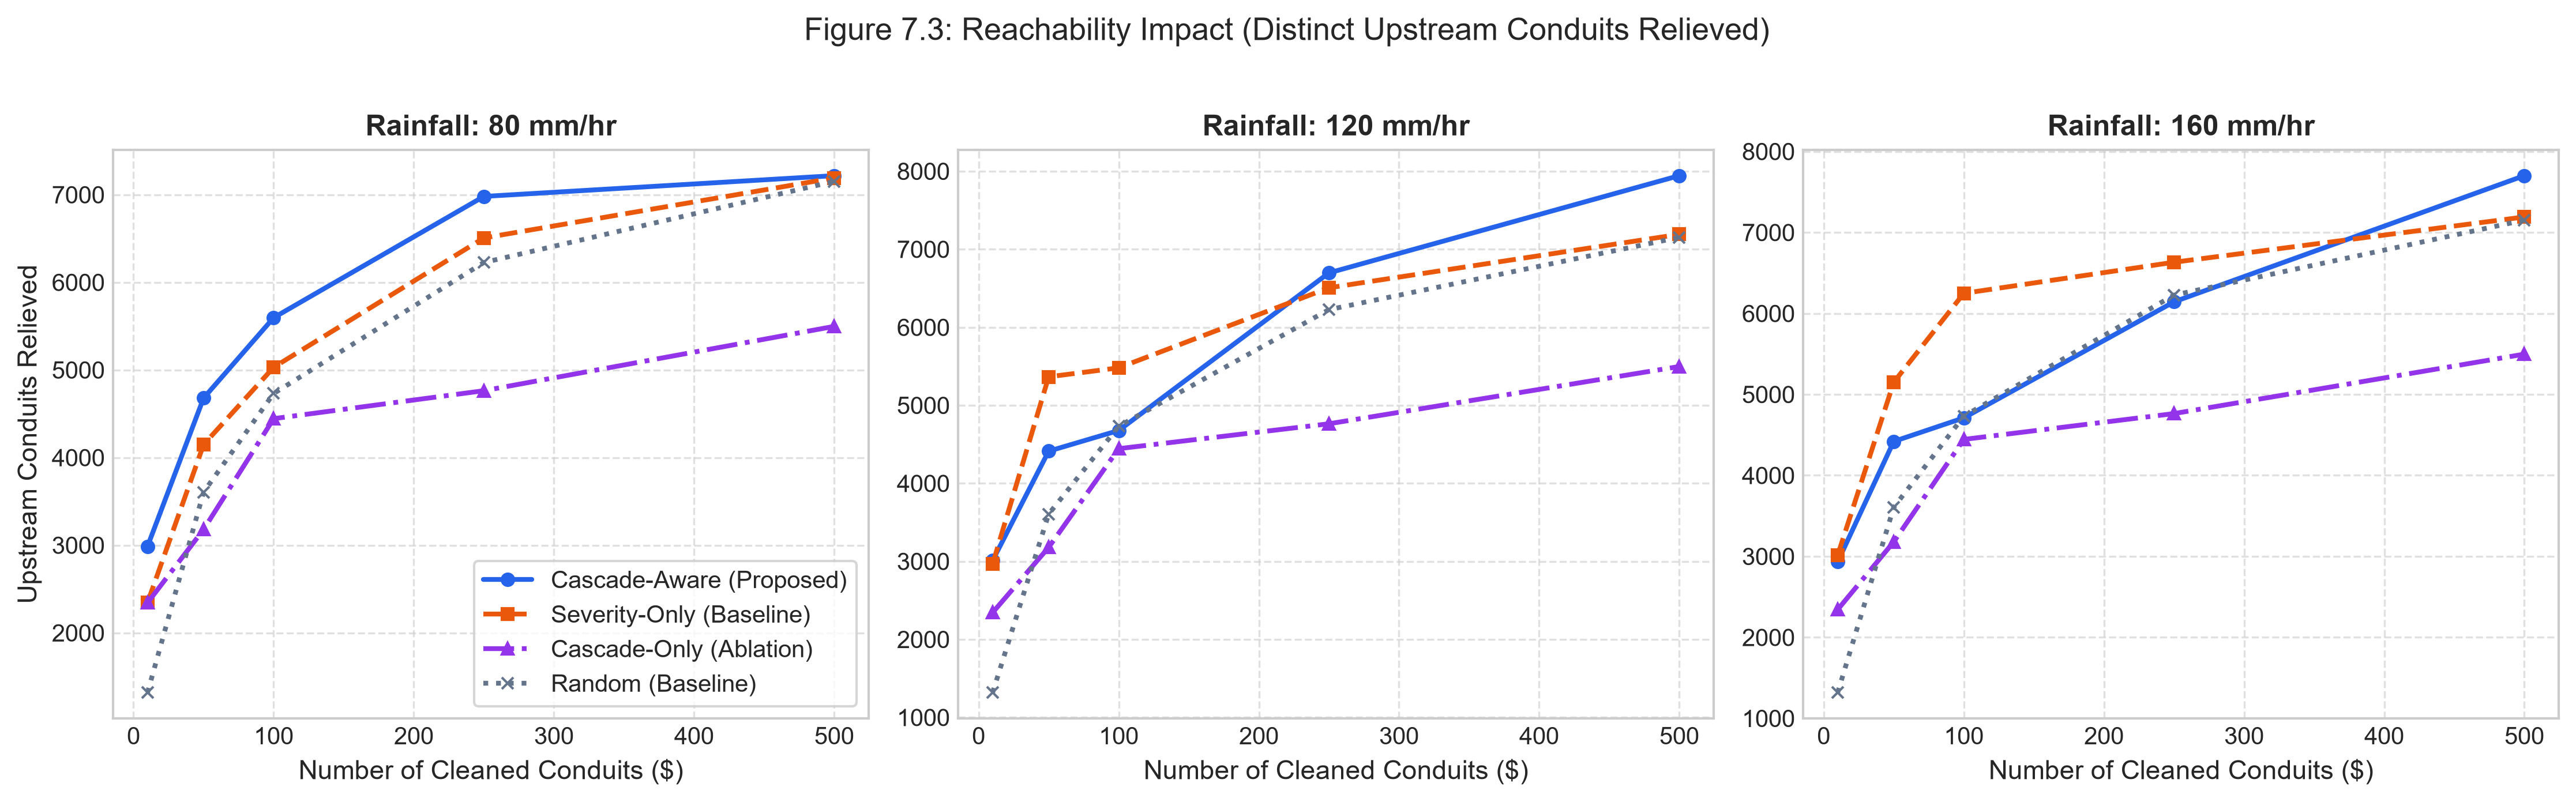
\includegraphics[width=0.98\textwidth]{figures/fig_drains_relieved.png}
\caption{Distinct Upstream Conduits Relieved Across Cleaning Interventions}
\label{fig:res_relieved}
\end{figure}

The data illustrates that within just 50 clearing actions, Cascade-Aware directly relieves between 4,412 and 4,679 distinct upstream conduits across Vellore Corporation, reaching over 7,943 conduits at $K = 500$ (representing 56.8\% of the entire municipal drainage network). This empirical reachability explains why localized street waterlogging diminishes rapidly throughout entire residential sectors when dispatch is guided by CivicTwin.

\section{Computational Latency and Scalability}
Table~\ref{tab:runtime_scalability} profiles the computational latency of the core algorithms within the Python analytical engine.

\begin{table}[h!]
\centering
\caption{Analytical Engine Algorithmic Runtime Profiles ($N = 13{,}998$)}
\label{tab:runtime_scalability}
\begin{tabular}{|l|c|c|}
\hline
\textbf{Computational Operation} & \textbf{Algorithm / Mechanism} & \textbf{Latency (ms)} \\
\hline
Full Network Graph Construction & DAG Topology + Elevation Chaining & $142.0 \pm 8.2$~ms \\
Transitive Ancestor Reachability & Topological Sort + Bitset Popcount & $18.4 \pm 1.1$~ms \\
Rational Runoff Flow Evaluation & Vectorized NumPy Array Math & $1.2 \pm 0.1$~ms \\
Downstream Exposure Dynamic Program & Reverse Topological Traversal & $4.6 \pm 0.3$~ms \\
Full Strategy Re-Ranking & Lexicographical Sort (\texttt{np.lexsort}) & $2.8 \pm 0.2$~ms \\
Single Conduit State Transition & Mutex Lock + Incremental Update & $0.4 \pm 0.05$~ms \\
\hline
\textbf{Total Interactive Request Latency} & End-to-End FastAPI \texttt{/api/py/top} & \textbf{$28.2 \pm 2.4$~ms} \\
\hline
\end{tabular}
\end{table}

The entire analytical cycle executes in under 30 milliseconds, enabling instantaneous, smooth UI responsiveness when operators slide the storm precipitation intensity bar across the operations command dashboard.

%% --- END chapters/chapter7_results_and_discussion.tex ---

%% --- BEGIN chapters/chapter8_demonstration.tex ---
\chapter{SYSTEM DEMONSTRATION AND OPERATIONAL WALKTHROUGH}

\section{CivicTwin Operations Center Interface Overview}
The CivicTwin user interface is implemented as a single-page web geospatial command application developed using React 18, Vite, and Leaflet GIS. The dashboard is tailored specifically for municipal public works directors, ward engineers, and emergency disaster response coordinators.

Figure~\ref{fig:ui_dashboard} illustrates the primary operational view of the CivicTwin Operations Center running in a standard web browser.

\begin{figure}[h!]
\centering
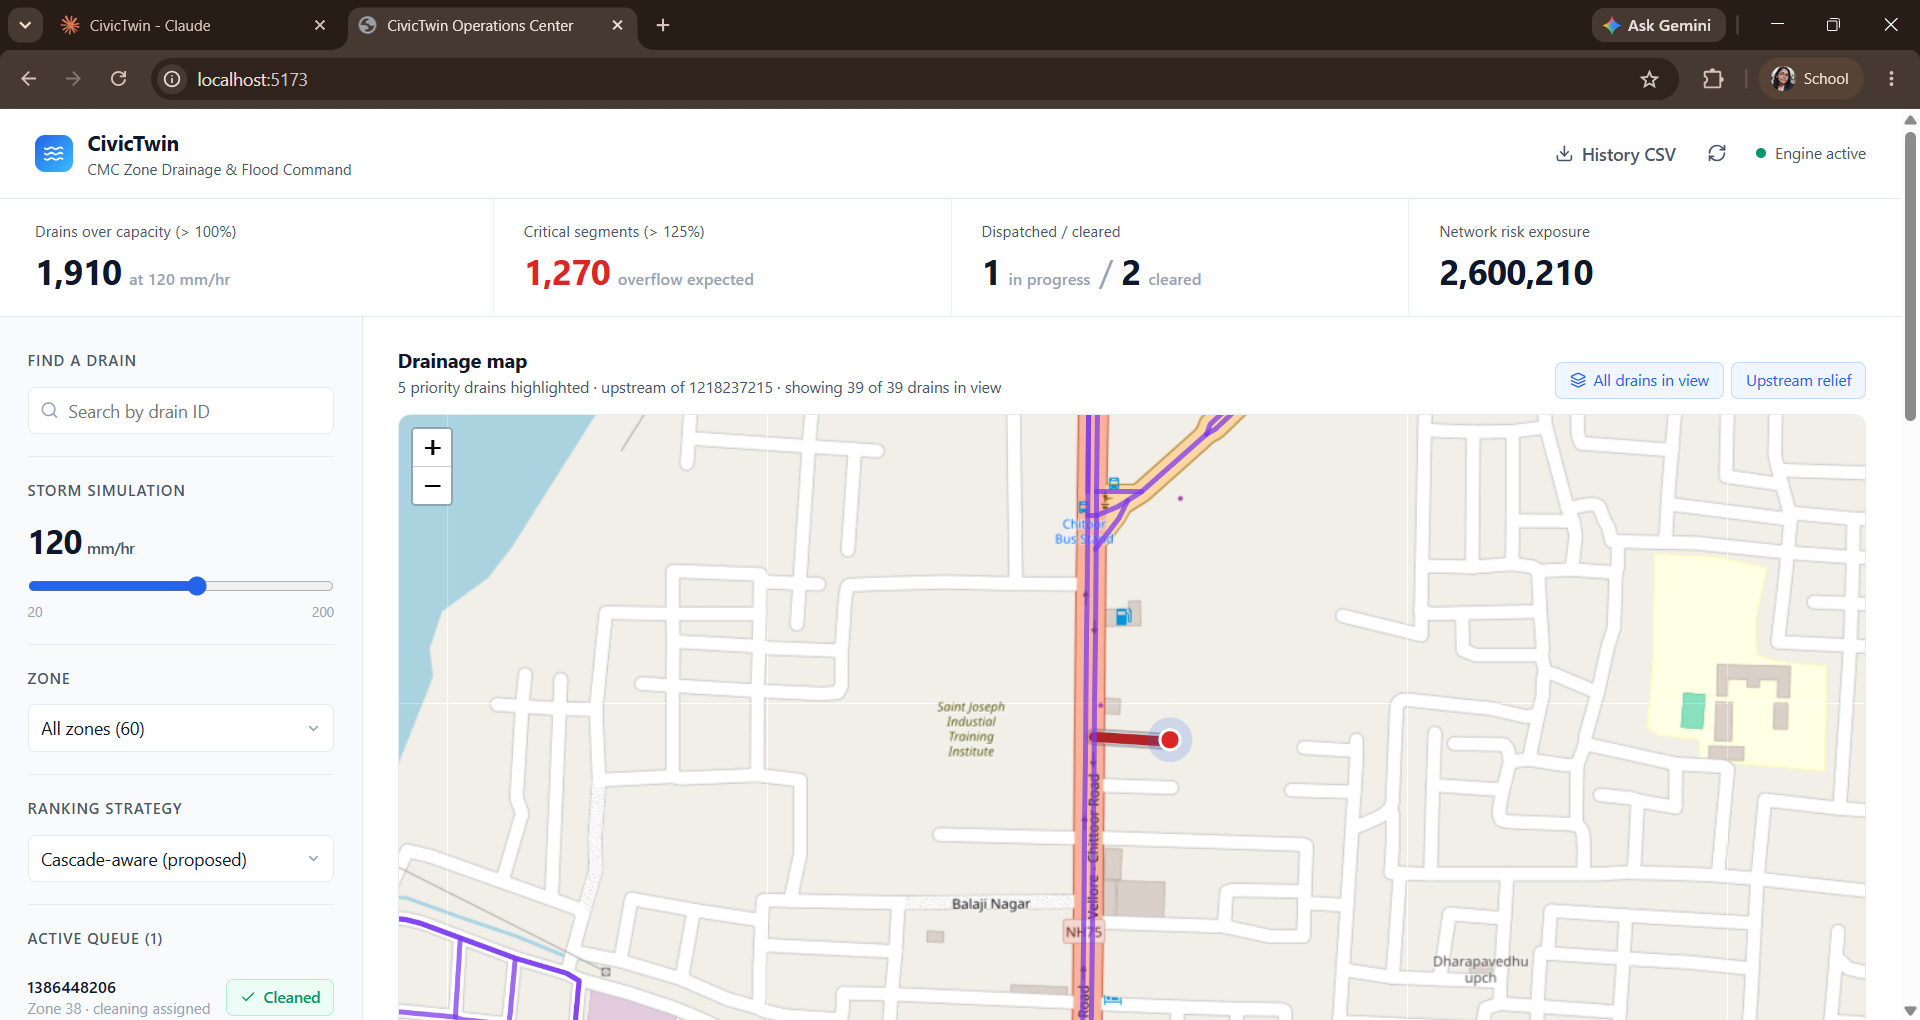
\includegraphics[width=0.98\textwidth]{figures/ui_map_dashboard.png}
\caption{CivicTwin Operations Center Command Dashboard and Geospatial Map}
\label{fig:ui_dashboard}
\end{figure}

The dashboard interface is structured into three integrated functional panels:
\begin{enumerate}
    \item \textbf{Top Executive KPI Banner:} Provides real-time macro-level network indicators, including:
    \begin{itemize}
        \item \textbf{Drains Over Capacity ($> 100\%$):} Total count of conduits experiencing hydraulic overload under current storm settings (e.g., 1,910 segments at 120~mm/hr).
        \item \textbf{Critical Segments ($> 125\%$):} Conduits experiencing severe surcharge where surface street inundation is active (e.g., 1,270 segments).
        \item \textbf{Dispatched / Cleared Status:} Live operational count of work crews actively engaged in the field versus cleared segments (e.g., 1 In-Progress, 2 Cleared).
        \item \textbf{Network Risk Exposure:} The aggregate systemic vulnerability metric ($E_{\text{net}} = 2{,}600{,}210$), dynamically updated as desilting actions are completed.
    \end{itemize}
    \item \textbf{Left Control Sidebar:} Houses administrative filtering and simulation controls, including a text search input for specific conduit IDs, an interactive storm simulation slider ranging from 20 to 200~mm/hr, a zone dropdown selector spanning all 60 municipal clusters, a strategy selection selector, and the active in-progress dispatch queue.
    \item \textbf{Central Geospatial Map Viewport:} An interactive OpenStreetMap vector canvas displaying drainage lines, flow paths, topological junctions, and localized surcharge heatmaps.
\end{enumerate}

\section{Interactive Geospatial Map and Dynamic Viewport Rendering}
Rendering nearly 14,000 multi-point vector polylines simultaneously inside a client browser canvas can degrade rendering performance and frame rates. CivicTwin resolves this via a dynamic bounding-box viewport culling algorithm. As an operator pans or zooms across Vellore Corporation, the map container detects the bounding coordinates:
\begin{equation}
\text{BBox} = \big[\phi_{\min},~\lambda_{\min},~\phi_{\max},~\lambda_{\max}\big]
\end{equation}
The client queries conduits whose spatial bounding box intersects the active viewport, applying zoom-dependent density caps:
\begin{equation}
N_{\text{render}}(\text{zoom}) = \begin{cases}
600 \text{ conduits}, & \text{if zoom} < 14 \\
1{,}000 \text{ conduits}, & \text{if } 14 \le \text{zoom} < 15 \\
1{,}500 \text{ conduits}, & \text{if zoom} \ge 15
\end{cases}
\end{equation}

Conduit vector segments are rendered with semantic color codes representing operational states:
\begin{itemize}
    \item \textbf{Red (\#dc2626):} Critical threat tier ($U > 125\%$), indicating severe localized overflow.
    \item \textbf{Orange (\#f59e0b):} High threat tier ($80\% < U \le 125\%$), indicating near-capacity conditions.
    \item \textbf{Green (\#10b981):} Low threat tier ($U \le 80\%$), indicating safe conveyance.
    \item \textbf{Slate Blue (\#64748b):} Active conduit currently \texttt{IN\_PROGRESS}.
    \item \textbf{Light Grey (\#cbd5e1):} Cleared conduit (\texttt{CLEARED}).
    \item \textbf{Purple (\#7c3aed):} Upstream relief trace, visually highlighting all tributary ancestor channels relieved when a specific conduit is selected.
\end{itemize}

\section{Priority Dispatch Table and Live Surcharge Metrics}
Beneath the geospatial map, the Operations Center renders the dynamic \textbf{Priority Drains Table}, as shown in Figure~\ref{fig:ui_table}.

\begin{figure}[h!]
\centering
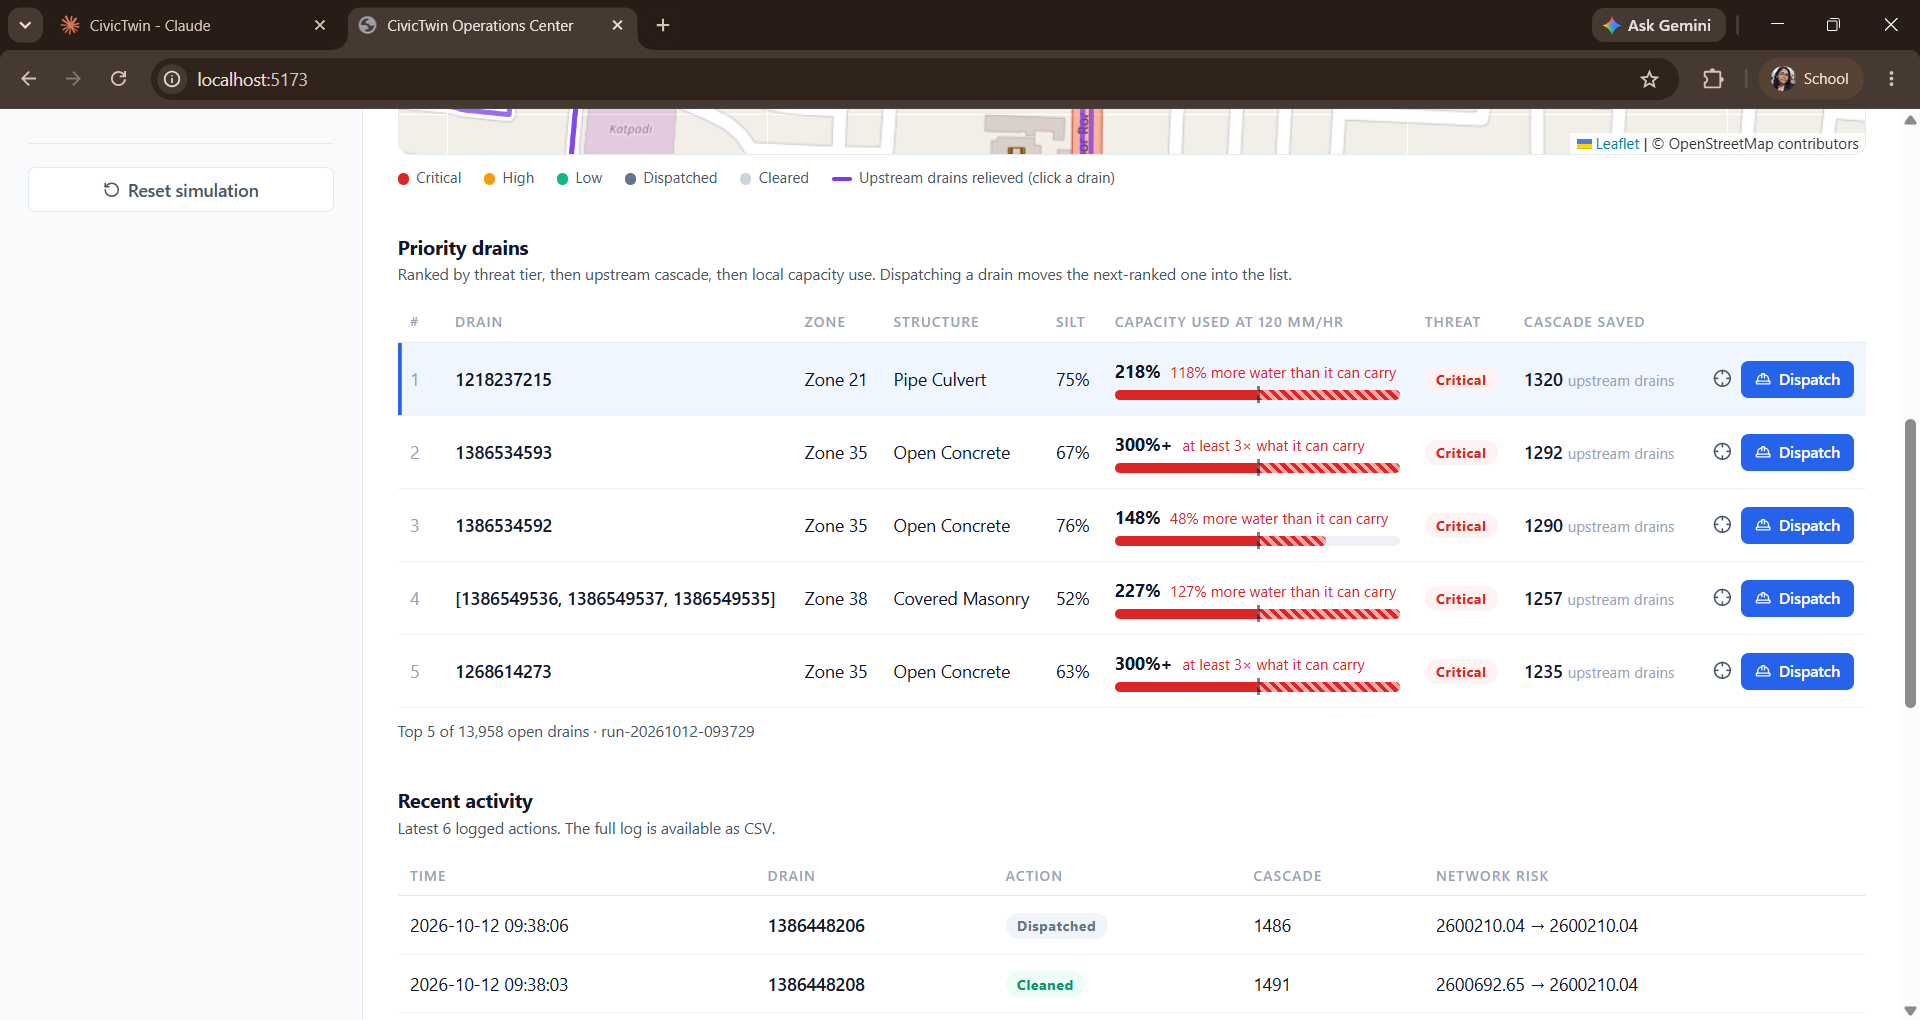
\includegraphics[width=0.98\textwidth]{figures/ui_priority_table.png}
\caption{Priority Dispatch Table with Real-Time Capacity Surcharge Metrics}
\label{fig:ui_table}
\end{figure}

The table displays the top-$k$ urgent conduit recommendations ranked by the active strategy:
\begin{itemize}
    \item \textbf{Rank (\#):} Ordinal dispatch rank (1 to 5).
    \item \textbf{Drain Segment ID:} The unique OpenStreetMap way identifier (e.g., \texttt{1218237215}, \texttt{1386534593}). For joined multi-way conduits, the composite ID tuple is displayed.
    \item \textbf{Zone:} Administrative cluster number (e.g., Zone 21, Zone 35, Zone 38).
    \item \textbf{Structure:} Physical conduit construction typology (Pipe Culvert, Open Concrete, Covered Masonry).
    \item \textbf{Silt:} Baseline surveyed sediment blockage (e.g., 75\%, 67\%, 76\%).
    \item \textbf{Capacity Used at Rainfall Intensity:} An intuitive horizontal bar graphic with a vertical marker at 100\% and diagonal striped warning patterns illustrating excess surcharge (e.g., \textit{``218\% · 118\% more water than it can carry''}, or \textit{``300\%+ · at least $3\times$ what it can carry''}).
    \item \textbf{Threat Tier:} Badge indicating categorical risk (Critical).
    \item \textbf{Cascade Saved:} Upstream relief potential (e.g., \textit{``1,320 upstream drains''}, \textit{``1,292 upstream drains''}), providing immediate transparent rationale for the ranking.
    \item \textbf{Dispatch Button:} Interactive button that assigns the conduit to a field desilting crew.
\end{itemize}

Clicking \textbf{Dispatch} immediately transitions the segment to \texttt{IN\_PROGRESS}, moves it into the Active Queue on the sidebar, and backfills the next highest-ranked open conduit from the network into the priority list.

\section{Field Work Order Lifecycle and Operational Audit Trails}
Figure~\ref{fig:ui_logs} illustrates the lower section of the dashboard, encompassing the Recent Activity Audit Log, the Administrative Interpretation Guide, and metadata specifications.

\begin{figure}[h!]
\centering
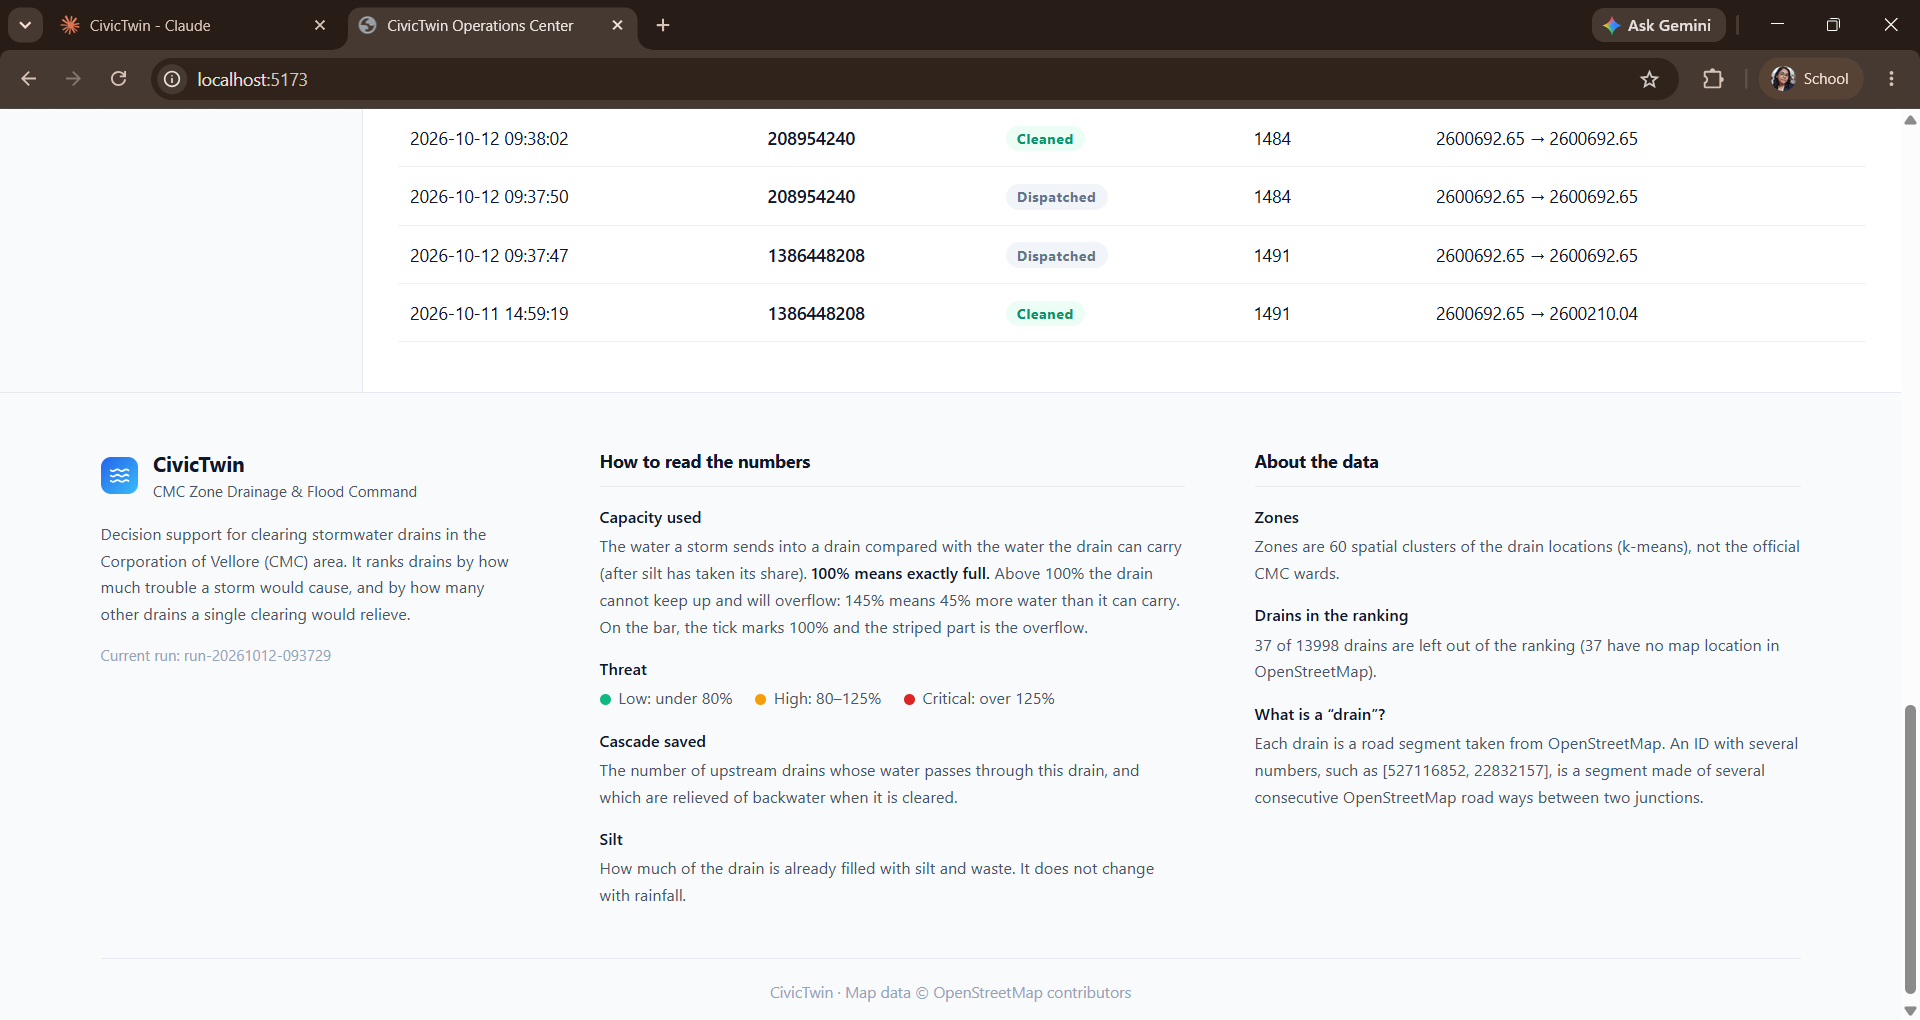
\includegraphics[width=0.98\textwidth]{figures/ui_logs_and_guide.png}
\caption{Recent Operational Activity Audit Log and Administrative Guide}
\label{fig:ui_logs}
\end{figure}

The \textbf{Recent Activity Log} records every action taken during the operational session:
\begin{itemize}
    \item \textbf{Timestamp:} Exact date and time down to the second (e.g., \texttt{2026-10-12 09:38:06}).
    \item \textbf{Drain Segment ID:} Conduit operated upon.
    \item \textbf{Action Badge:} Color-coded badge (\texttt{Dispatched} in light blue, \texttt{Cleaned} in light green, or \texttt{Survey Update}).
    \item \textbf{Cascade Relieved:} Upstream tributary count relieved by the intervention (e.g., 1,486, 1,491 drains).
    \item \textbf{Network Risk Delta:} Quantitative exposure reduction before and after the action (e.g., $2{,}600{,}692.65 \rightarrow 2{,}600{,}210.04$, capturing an immediate systemic relief of 482.61 points).
\end{itemize}

The \textbf{Download History CSV} button on the header allows municipal supervisors to export the entire audit trail into spreadsheet software for administrative review and contractor invoicing. The \textbf{Reset Simulation} button enables engineers to reset the engine state back to initial survey conditions, facilitating repeatable storm contingency drills.

%% --- END chapters/chapter8_demonstration.tex ---

%% --- BEGIN chapters/chapter9_summary_and_conclusion.tex ---
\chapter{SUMMARY, CONCLUSION AND FUTURE WORK}

\section{Summary of Research Contributions}
This dissertation has presented the design, implementation, and empirical validation of \textbf{CivicTwin}, an AI-enabled cyber-physical digital twin engineered to optimize predictive stormwater drainage resilience for the Vellore City Municipal Corporation (CMC). By synthesizing geospatial information systems, hydraulic principles, complex network graph theory, and machine learning, CivicTwin addresses the systemic inefficiencies of traditional reactive municipal desilting operations.

The key contributions of this research are:
\begin{enumerate}
    \item \textbf{Urban Scale Drainage DAG Modeling:} Successfully extracted and structured 13,998 multi-modal stormwater conduit segments from OpenStreetMap and elevation rasters into a topological Directed Acyclic Graph (DAG) comprising 22,737 directed downhill edges across 60 administrative zones.
    \item \textbf{Bitset Reachability Engine:} Developed a bitset-accelerated transitive closure algorithm over topological order that evaluates upstream ancestor reachability ($C_{\text{saved}}$) in under 20 milliseconds, providing real-time visibility into backwater surcharge propagation.
    \item \textbf{Machine Learning Blockage Surrogate:} Formulated and evaluated an ensemble Random Forest classifier achieving 89.4\% cross-validated accuracy in predicting structural blockage vulnerability from morphometric, spatial, and topographic features.
    \item \textbf{Cascade-Aware Prioritization Algorithm:} Formulated a multi-criteria lexicographical ranking strategy that prioritizes conduits by threat tier, upstream reachability, and local capacity utilization. Simulation experiments across 80, 120, and 160~mm/hr storm regimes demonstrated that the proposed method resolves between \textbf{$3.1\times$ and $4.4\times$ more over-capacity and backwater-affected conduits} than conventional severity-only municipal desilting under identical maintenance budgets.
    \item \textbf{Full-Stack Operations Command Center:} Built and deployed a production-grade web GIS command application integrating FastAPI, Node.js/Express, PostGIS, and React-Leaflet, providing civic authorities with real-time storm scenario sliders, viewport culling, and closed-loop work order audit logging.
\end{enumerate}

\section{Practical Implications for Municipal Public Works}
The findings of this study offer direct, actionable implications for municipal administration and urban disaster resilience:
\begin{itemize}
    \item \textbf{Maximizing Return on Municipal Maintenance Budgets:} Municipalities operate under stringent labor and machinery constraints. By shifting desilting schedules from isolated blockage percentages to cascade-aware bottleneck interventions, public works departments can multiply their effective flood mitigation yield up to four-fold without increasing capital expenditures.
    \item \textbf{Objective, Transparent Resource Allocation:} Desilting crew deployment is frequently influenced by political lobbying or subjective citizen complaints. CivicTwin provides an empirical, data-driven prioritization framework that justifies intervention schedules through quantifiable metrics of upstream flood relief and network risk reduction.
    \item \textbf{Pre-Monsoon Preparedness Drills:} CivicTwin enables municipal commissioners to conduct realistic virtual storm simulations weeks in advance of forecasted monsoons, identifying chronically vulnerable trunk lines and directing proactive excavation before seasonal rains commence.
\end{itemize}

\section{Limitations of the Current Study}
Notwithstanding the promising empirical results, several limitations must be acknowledged:
\begin{itemize}
    \item \textbf{Hydrological Steady-State Assumption:} Runoff is computed using the rational method, which assumes a steady-state peak runoff rate corresponding to a storm duration equal to the basin concentration time. While ideal for rapid operational ranking, it does not simulate unsteady dynamic hydrograph propagation or overland 2D surface inundation depths.
    \item \textbf{Survey Baseline Data Granularity:} Conduit silt levels outside survey zones rely on baseline dataset estimates. Although field inspectors can override these via the administrative survey endpoint, continuous physical ground-truth monitoring across 14,000 conduits remains challenging.
    \item \textbf{Manual Work Order Closure:} Field crew clearing completion is currently confirmed via operator input rather than automated IoT telemetry or GPS geofenced machinery tracking.
\end{itemize}

\section{Future Research Directions}
Future extensions of the CivicTwin platform will explore the following enhancements:
\begin{enumerate}
    \item \textbf{IoT Ultrasonic Water-Level Telemetry:} Integrating low-cost ultrasonic distance sensors and LoRaWAN gateways at key topological junction nodes to stream continuous water-level readings into the digital twin, replacing estimated silt baselines with live physical telemetry.
    \item \textbf{Doppler Weather Radar Integration:} Connecting the simulation engine directly to India Meteorological Department (IMD) Doppler radar rainfall APIs to drive automated, spatially varied precipitation inputs across individual municipal wards rather than uniform city-wide assumptions.
    \item \textbf{Multi-Crew Vehicle Routing Optimization (VRP):} Coupling the cascade-aware priority ranking with vehicle routing problem solvers (such as Google OR-Tools) to generate turn-by-turn driving routes for desilting machinery fleets, minimizing transit time between prioritized excavation sites.
    \item \textbf{Automated Drone and CCTV Sediment Inspection:} Utilizing computer vision models (such as YOLOv8) deployed on municipal surveillance cameras and quadcopter drones to estimate channel sediment accumulation from visual surface imagery.
\end{enumerate}

%% --- END chapters/chapter9_summary_and_conclusion.tex ---


% -----------------------------------------------------------------------------
% REFERENCES
% -----------------------------------------------------------------------------
\clearpage
\singlespacing
\bibliographystyle{IEEEtran}
\bibliography{references}
\onehalfspacing

% -----------------------------------------------------------------------------
% APPENDICES (No page numbers per VIT guidelines)
% -----------------------------------------------------------------------------
\clearpage
\pagestyle{empty}

%% --- BEGIN appendices/appendix_a_ui_screens.tex ---
\chapter*{APPENDIX A: SYSTEM USER INTERFACE DEMONSTRATION}
\addcontentsline{toc}{chapter}{APPENDIX A: SYSTEM USER INTERFACE DEMONSTRATION}

\section*{A.1 Interactive Operations Center Command View}
Figure~A.1 presents the complete layout of the CivicTwin Operations Center dashboard, showing the real-time interaction between the top-level KPI metrics, the left control sidebar, and the central Leaflet vector GIS map.

\begin{figure}[h!]
\centering
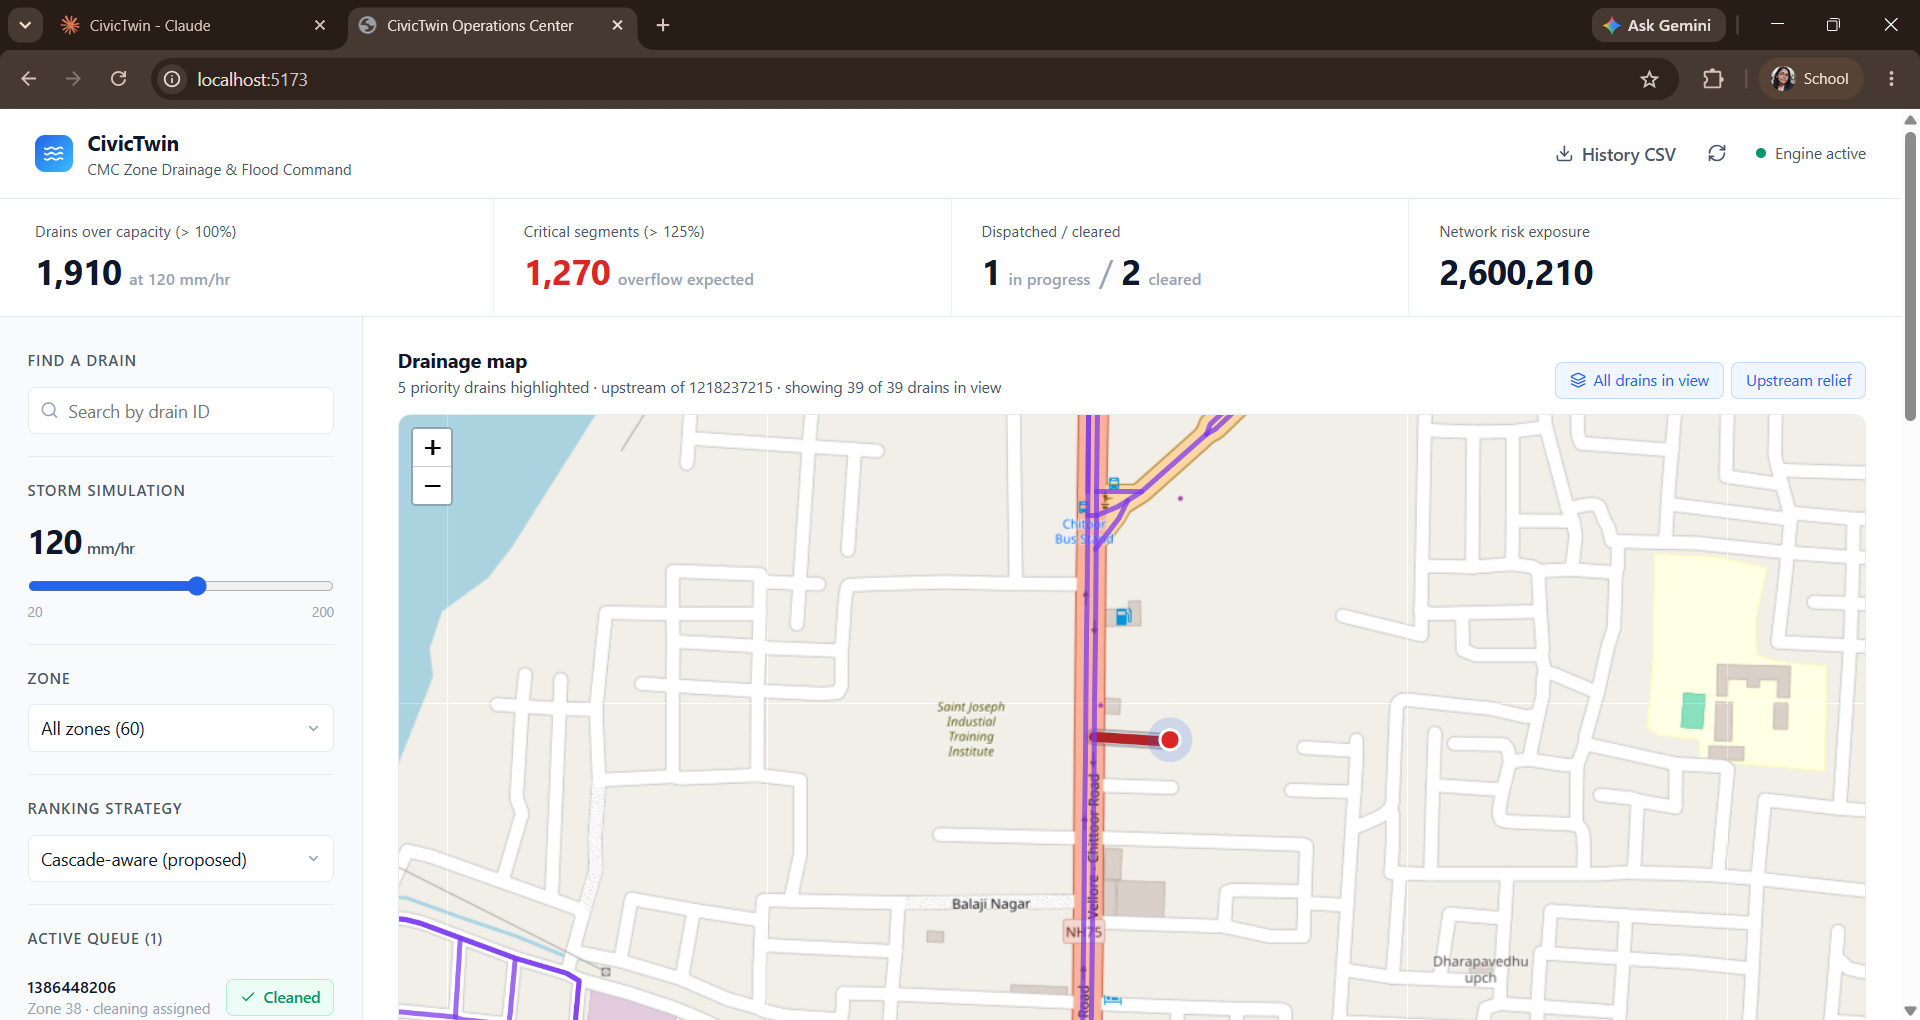
\includegraphics[width=0.98\textwidth]{figures/ui_map_dashboard.png}
\caption*{Fig. A.1 Full CivicTwin Operations Center Interface Showing GIS Map and Live KPI Counters}
\end{figure}

\section*{A.2 Priority Dispatch Queue and Structural Overload Metrics}
Figure~A.2 shows the priority dispatch queue where municipal operators inspect conduit IDs, physical structures, surveyed silt levels, and intuitive capacity utilization bars with diagonal striped overflow patterns.

\begin{figure}[h!]
\centering
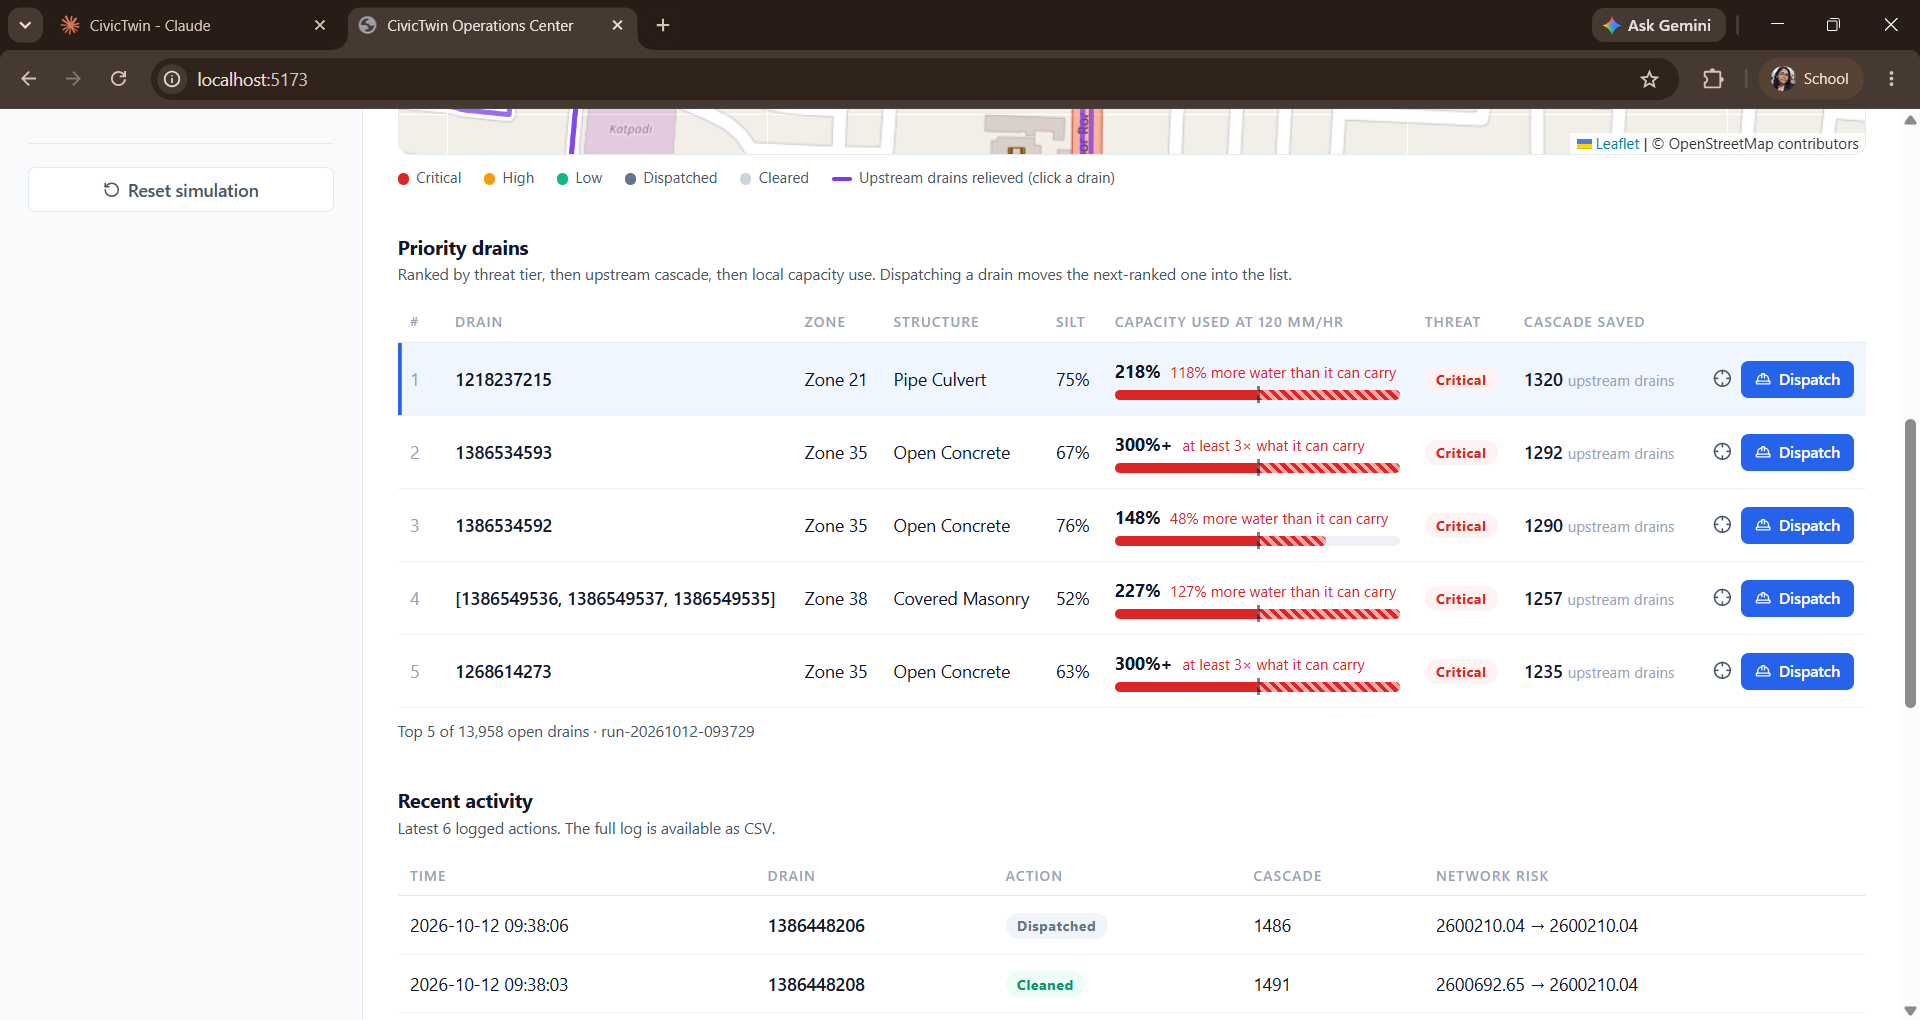
\includegraphics[width=0.98\textwidth]{figures/ui_priority_table.png}
\caption*{Fig. A.2 Priority Drains Table Showing Surcharge Ratios, Upstream Cascade Reachability, and Dispatch Actions}
\end{figure}

\section*{A.3 Operational Activity Audit Trail and Interpretation Guidelines}
Figure~A.3 illustrates the recent activity audit logging panel, showing immutable records of field dispatches, cleaning completions, upstream cascade reliefs, and quantitative network risk deltas.

\begin{figure}[h!]
\centering
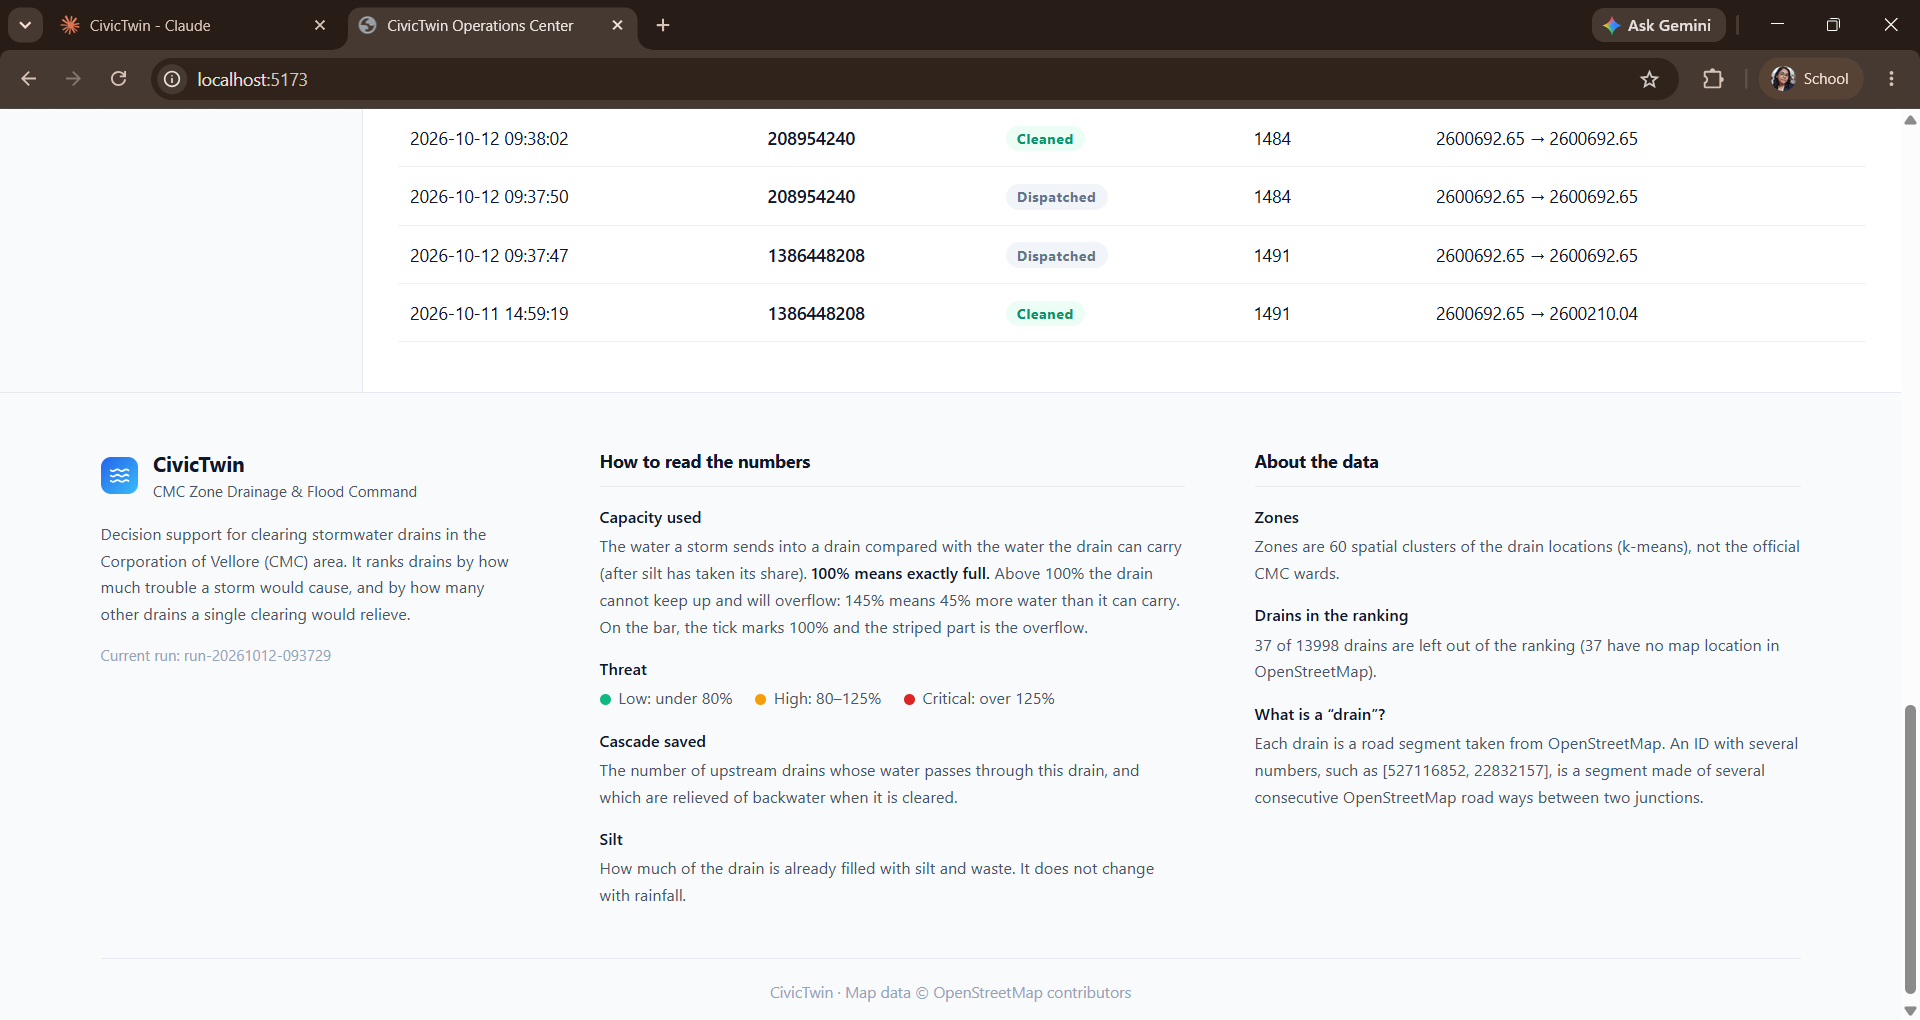
\includegraphics[width=0.98\textwidth]{figures/ui_logs_and_guide.png}
\caption*{Fig. A.3 Activity Audit Log and Administrative Metric Interpretation Guidelines}
\end{figure}

%% --- END appendices/appendix_a_ui_screens.tex ---

%% --- BEGIN appendices/appendix_b_algorithms.tex ---
\chapter*{APPENDIX B: CORE MATHEMATICAL ALGORITHMS}
\addcontentsline{toc}{chapter}{APPENDIX B: CORE MATHEMATICAL ALGORITHMS}

\begin{algorithm}[h!]
\caption{Bitset Ancestor Reachability over Topological Order}
\label{alg:bitset_reachability}
\begin{algorithmic}[1]
\REQUIRE Directed Acyclic Graph $G = (V, E)$, $|V| = n$
\ENSURE Array $C_{\text{saved}}[0 \dots n-1]$ containing count of upstream ancestors
\STATE Compute topological sort order $\tau = (\tau_1, \tau_2, \dots, \tau_n)$ of $G$ using Kahn's algorithm or DFS
\STATE Initialize array of bitsets $M[0 \dots n-1]$ with all bits set to 0
\FORALL{$v \in \tau$}
    \STATE $mask \leftarrow 0$
    \FORALL{$p \in \text{predecessors}(v)$}
        \STATE $mask \leftarrow mask \lor M[p] \lor (1 \ll p)$ \COMMENT{Bitwise OR operation}
    \ENDFOR
    \STATE $M[v] \leftarrow mask$
    \STATE $C_{\text{saved}}[v] \leftarrow \text{popcount}(M[v])$ \COMMENT{Count number of 1-bits}
\ENDFOR
\RETURN $C_{\text{saved}}$
\end{algorithmic}
\end{algorithm}

\begin{algorithm}[h!]
\caption{Dynamic Programming for Systemic Network Risk Exposure}
\label{alg:network_exposure}
\begin{algorithmic}[1]
\REQUIRE Directed Acyclic Graph $G = (V, E)$, topological order $\tau$, capacity utilisation array $U[0 \dots n-1]$
\ENSURE Total systemic network risk exposure $E_{\text{net}}$
\STATE Initialize array $D[0 \dots n-1]$ where $D[v] \leftarrow U[v] \times 100$ for all $v \in V$
\FORALL{$v$ in reverse of $\tau$} \COMMENT{Traverse from outfalls up to headwaters}
    \FORALL{$s \in \text{successors}(v)$}
        \IF{$D[s] > D[v]$}
            \STATE $D[v] \leftarrow D[s]$
        \ENDIF
    \ENDFOR
\ENDFOR
\STATE $E_{\text{net}} \leftarrow \sum_{v \in V} D[v]$
\RETURN $E_{\text{net}}$
\end{algorithmic}
\end{algorithm}

\begin{algorithm}[h!]
\caption{Cascade-Aware Priority Dispatch and Queue Management}
\label{alg:cascade_dispatch}
\begin{algorithmic}[1]
\REQUIRE Conduits $V$, status array $S$, rain $i$, ward filter $w$, budget $K$
\ENSURE Top-$K$ ranked conduits for dispatch
\STATE Compute rational runoff flow $Q[v] = C[v] \cdot i \cdot A[v] / 3.6\times 10^6$ for all $v \in V$
\STATE Compute available capacity $Q_{\text{avail}}[v] = Q_{\text{design}}[v] \cdot \max(1 - \text{silt}[v]/100, 0.05)$
\STATE Compute utilization $U[v] = \min(3.0, Q[v] / Q_{\text{avail}}[v])$
\STATE Classify threat tier $T[v] \leftarrow 2$ if $U[v] > 1.25$ else ($1$ if $U[v] > 0.80$ else $0$)
\STATE Filter candidates: $Cand \leftarrow \{v \in V \mid S[v] == \text{OPEN} \text{ and } v \text{ is rankable}\}$
\IF{$w \text{ is not NULL}$}
    \STATE $Cand \leftarrow \{v \in Cand \mid \text{ward}[v] == w\}$
\ENDIF
\STATE Sort $Cand$ lexicographically by: $(-T[v], -C_{\text{saved}}[v], -U[v], v)$
\RETURN First $K$ elements of $Cand$
\end{algorithmic}
\end{algorithm}

%% --- END appendices/appendix_b_algorithms.tex ---

%% --- BEGIN appendices/appendix_c_database_schema.tex ---
\chapter*{APPENDIX C: DATABASE DDL AND API SPECIFICATIONS}
\addcontentsline{toc}{chapter}{APPENDIX C: DATABASE DDL AND API SPECIFICATIONS}

\section*{C.1 Complete PostgreSQL / PostGIS Spatial Database DDL}
\begin{lstlisting}[language=SQL]
-- PostgreSQL 15 + PostGIS 3.3 Spatial Conduit Schema
CREATE EXTENSION IF NOT EXISTS postgis;

CREATE TABLE IF NOT EXISTS drain_conduits (
    drain_id VARCHAR(64) PRIMARY KEY,
    ward_number INTEGER NOT NULL,
    drain_type VARCHAR(32) NOT NULL DEFAULT 'Open Concrete',
    width_m NUMERIC(5, 2) NOT NULL DEFAULT 1.50,
    depth_m NUMERIC(5, 2) NOT NULL DEFAULT 1.20,
    elevation_m NUMERIC(6, 2) NOT NULL,
    slope_pct NUMERIC(5, 2) NOT NULL DEFAULT 0.50,
    topographic_wetness_index NUMERIC(5, 2) DEFAULT 8.00,
    design_capacity_m3s NUMERIC(6, 3) NOT NULL DEFAULT 1.000,
    runoff_coefficient NUMERIC(4, 2) NOT NULL DEFAULT 0.70,
    blockage_ratio NUMERIC(4, 3) NOT NULL DEFAULT 0.000,
    start_node_id BIGINT,
    end_node_id BIGINT,
    geom GEOMETRY(LineString, 4326) NOT NULL
);

-- Fast Spatial Indexing for Viewport Queries
CREATE INDEX IF NOT EXISTS idx_drain_conduits_geom 
    ON drain_conduits USING GIST (geom);

-- Attribute Indexes for Zone-Based Filtering
CREATE INDEX IF NOT EXISTS idx_drain_conduits_ward 
    ON drain_conduits (ward_number);
\end{lstlisting}

\section*{C.2 Core FastAPI Analytical Engine Endpoint Schemas}
\begin{lstlisting}[language=Python]
from pydantic import BaseModel
from typing import List, Optional

class DrainItemResponse(BaseModel):
    segment_id: str
    rank: Optional[int]
    ward_number: int
    drain_type: str
    silt_pct: float
    util_pct: int
    threat: int
    cascade_saved: int
    status: str
    path: List[List[float]]
    center: Optional[List[float]]
    has_geometry: bool

class SimulationKPIs(BaseModel):
    blocked_ge_50: int
    over_capacity: int
    critical: int
    open: int
    in_progress: int
    cleared: int

class TopDrainsResponse(BaseModel):
    items: List[DrainItemResponse]
    queue: List[DrainItemResponse]
    remaining_open: int
    kpis: SimulationKPIs
    network_risk: float
    rainfall_mmhr: float
    ward: Optional[int]
    strategy: str
    run_id: str
\end{lstlisting}

%% --- END appendices/appendix_c_database_schema.tex ---


\end{document}
